\documentclass[twoside]{book}

% Packages required by doxygen
\usepackage{fixltx2e}
\usepackage{calc}
\usepackage{doxygen}
\usepackage{graphicx}
\usepackage[utf8]{inputenc}
\usepackage{makeidx}
\usepackage{multicol}
\usepackage{multirow}
\PassOptionsToPackage{warn}{textcomp}
\usepackage{textcomp}
\usepackage[nointegrals]{wasysym}
\usepackage[table]{xcolor}

% Font selection
\usepackage[T1]{fontenc}
\usepackage{mathptmx}
\usepackage[scaled=.90]{helvet}
\usepackage{courier}
\usepackage{amssymb}
\usepackage{sectsty}
\renewcommand{\familydefault}{\sfdefault}
\allsectionsfont{%
  \fontseries{bc}\selectfont%
  \color{darkgray}%
}
\renewcommand{\DoxyLabelFont}{%
  \fontseries{bc}\selectfont%
  \color{darkgray}%
}
\newcommand{\+}{\discretionary{\mbox{\scriptsize$\hookleftarrow$}}{}{}}

% Page & text layout
\usepackage{geometry}
\geometry{%
  a4paper,%
  top=2.5cm,%
  bottom=2.5cm,%
  left=2.5cm,%
  right=2.5cm%
}
\tolerance=750
\hfuzz=15pt
\hbadness=750
\setlength{\emergencystretch}{15pt}
\setlength{\parindent}{0cm}
\setlength{\parskip}{0.2cm}
\makeatletter
\renewcommand{\paragraph}{%
  \@startsection{paragraph}{4}{0ex}{-1.0ex}{1.0ex}{%
    \normalfont\normalsize\bfseries\SS@parafont%
  }%
}
\renewcommand{\subparagraph}{%
  \@startsection{subparagraph}{5}{0ex}{-1.0ex}{1.0ex}{%
    \normalfont\normalsize\bfseries\SS@subparafont%
  }%
}
\makeatother

% Headers & footers
\usepackage{fancyhdr}
\pagestyle{fancyplain}
\fancyhead[LE]{\fancyplain{}{\bfseries\thepage}}
\fancyhead[CE]{\fancyplain{}{}}
\fancyhead[RE]{\fancyplain{}{\bfseries\leftmark}}
\fancyhead[LO]{\fancyplain{}{\bfseries\rightmark}}
\fancyhead[CO]{\fancyplain{}{}}
\fancyhead[RO]{\fancyplain{}{\bfseries\thepage}}
\fancyfoot[LE]{\fancyplain{}{}}
\fancyfoot[CE]{\fancyplain{}{}}
\fancyfoot[RE]{\fancyplain{}{\bfseries\scriptsize Generated on Sun Dec 7 2014 23\+:54\+:35 for C\+List by Doxygen }}
\fancyfoot[LO]{\fancyplain{}{\bfseries\scriptsize Generated on Sun Dec 7 2014 23\+:54\+:35 for C\+List by Doxygen }}
\fancyfoot[CO]{\fancyplain{}{}}
\fancyfoot[RO]{\fancyplain{}{}}
\renewcommand{\footrulewidth}{0.4pt}
\renewcommand{\chaptermark}[1]{%
  \markboth{#1}{}%
}
\renewcommand{\sectionmark}[1]{%
  \markright{\thesection\ #1}%
}

% Indices & bibliography
\usepackage{natbib}
\usepackage[titles]{tocloft}
\setcounter{tocdepth}{3}
\setcounter{secnumdepth}{5}
\makeindex

% Hyperlinks (required, but should be loaded last)
\usepackage{ifpdf}
\ifpdf
  \usepackage[pdftex,pagebackref=true]{hyperref}
\else
  \usepackage[ps2pdf,pagebackref=true]{hyperref}
\fi
\hypersetup{%
  colorlinks=true,%
  linkcolor=blue,%
  citecolor=blue,%
  unicode%
}

% Custom commands
\newcommand{\clearemptydoublepage}{%
  \newpage{\pagestyle{empty}\cleardoublepage}%
}


%===== C O N T E N T S =====

\begin{document}

% Titlepage & ToC
\hypersetup{pageanchor=false,
             bookmarks=true,
             bookmarksnumbered=true,
             pdfencoding=unicode
            }
\pagenumbering{roman}
\begin{titlepage}
\vspace*{7cm}
\begin{center}%
{\Large C\+List \\[1ex]\large 1.\+0 }\\
\vspace*{1cm}
{\large Generated by Doxygen 1.8.8}\\
\vspace*{0.5cm}
{\small Sun Dec 7 2014 23:54:35}\\
\end{center}
\end{titlepage}
\clearemptydoublepage
\tableofcontents
\clearemptydoublepage
\pagenumbering{arabic}
\hypersetup{pageanchor=true}

%--- Begin generated contents ---
\chapter{Documention for the class \char`\"{}\+C\+List\char`\"{}}
\label{index}\hypertarget{index}{}This class have for goal to approach the most class list from the S\+T\+L. So for this reason we choose to implement a double-\/linked list and we think it's easier for users to work with double linked list. We implement the most part of the list class functions like emplace, insert, ... and we implement iterator to provide a simple way to browse the list. 
\chapter{Hierarchical Index}
\section{Class Hierarchy}
This inheritance list is sorted roughly, but not completely, alphabetically\+:\begin{DoxyCompactList}
\item C\+Const\+Iter\+Base\begin{DoxyCompactList}
\item \contentsline{section}{ns\+Sd\+D\+:\+:C\+List$<$ T $>$\+:\+:C\+Const\+Iterator$<$ T $>$}{\pageref{structnsSdD_1_1CList_1_1CConstIterator}}{}
\end{DoxyCompactList}
\item C\+Iter\+Base\begin{DoxyCompactList}
\item \contentsline{section}{ns\+Sd\+D\+:\+:C\+List$<$ T $>$\+:\+:C\+Iterator$<$ T $>$}{\pageref{structnsSdD_1_1CList_1_1CIterator}}{}
\end{DoxyCompactList}
\item \contentsline{section}{ns\+Sd\+D\+:\+:C\+List$<$ T $>$}{\pageref{classnsSdD_1_1CList}}{}
\item \contentsline{section}{ns\+Sd\+D\+:\+:C\+List$<$ T $>$\+:\+:C\+Node}{\pageref{classnsSdD_1_1CList_1_1CNode}}{}
\item \contentsline{section}{ns\+Tests\+:\+:C\+Tests}{\pageref{classnsTests_1_1CTests}}{}
\item \contentsline{section}{ns\+Tests\+:\+:C\+Value\+Provider$<$ T $>$}{\pageref{classnsTests_1_1CValueProvider}}{}
\item \contentsline{section}{ns\+Tests\+:\+:C\+Value\+Provider$<$ int $>$}{\pageref{classnsTests_1_1CValueProvider_3_01int_01_4}}{}
\item \contentsline{section}{ns\+Tests\+:\+:C\+Value\+Provider$<$ std\+:\+:shared\+\_\+ptr$<$ T $>$ $>$}{\pageref{classnsTests_1_1CValueProvider_3_01std_1_1shared__ptr_3_01T_01_4_01_4}}{}
\item \contentsline{section}{ns\+Tests\+:\+:C\+Value\+Provider$<$ T $\ast$ $>$}{\pageref{classnsTests_1_1CValueProvider_3_01T_01_5_01_4}}{}
\item \contentsline{section}{ns\+Tests\+:\+:C\+Value\+Provider$<$ Test\+Class $>$}{\pageref{classnsTests_1_1CValueProvider_3_01TestClass_01_4}}{}
\item \contentsline{section}{ns\+Tests\+:\+:Test\+Class}{\pageref{classnsTests_1_1TestClass}}{}
\end{DoxyCompactList}

\chapter{Class Index}
\section{Class List}
Here are the classes, structs, unions and interfaces with brief descriptions\+:\begin{DoxyCompactList}
\item\contentsline{section}{\hyperlink{structnsSdD_1_1CList_1_1CConstIterator}{ns\+Sd\+D\+::\+C\+List$<$ T $>$\+::\+C\+Const\+Iterator$<$ T $>$} }{\pageref{structnsSdD_1_1CList_1_1CConstIterator}}{}
\item\contentsline{section}{\hyperlink{structnsSdD_1_1CList_1_1CIterator}{ns\+Sd\+D\+::\+C\+List$<$ T $>$\+::\+C\+Iterator$<$ T $>$} \\*This class is a personnal implementation of iterator for our class \hyperlink{classnsSdD_1_1CList}{C\+List}. We provide the essential function to work with us. We implement bidirectionnal iterator because we choose to use a double-\/linked list }{\pageref{structnsSdD_1_1CList_1_1CIterator}}{}
\item\contentsline{section}{\hyperlink{classnsSdD_1_1CList}{ns\+Sd\+D\+::\+C\+List$<$ T $>$} \\*\hyperlink{classnsSdD_1_1CList}{C\+List} is the main class of our work, it's develop in order to be the most close to the original std\+::list In this idea we choose to make a double-\/linked list, in that way we can use bidirectional iterator and have a stl compliant \hyperlink{classnsSdD_1_1CList}{C\+List}. During the development process we choose to work in T\+D\+D (Test Driven Development) in order to have the least bugs possible }{\pageref{classnsSdD_1_1CList}}{}
\item\contentsline{section}{\hyperlink{classnsSdD_1_1CList_1_1CNode}{ns\+Sd\+D\+::\+C\+List$<$ T $>$\+::\+C\+Node} }{\pageref{classnsSdD_1_1CList_1_1CNode}}{}
\item\contentsline{section}{\hyperlink{classnsTests_1_1CTests}{ns\+Tests\+::\+C\+Tests} }{\pageref{classnsTests_1_1CTests}}{}
\item\contentsline{section}{\hyperlink{classnsTests_1_1CValueProvider}{ns\+Tests\+::\+C\+Value\+Provider$<$ T $>$} \\*\hyperlink{classnsTests_1_1CValueProvider}{C\+Value\+Provider} provides semi-\/random values for tested classes.. }{\pageref{classnsTests_1_1CValueProvider}}{}
\item\contentsline{section}{\hyperlink{classnsTests_1_1CValueProvider_3_01int_01_4}{ns\+Tests\+::\+C\+Value\+Provider$<$ int $>$} }{\pageref{classnsTests_1_1CValueProvider_3_01int_01_4}}{}
\item\contentsline{section}{\hyperlink{classnsTests_1_1CValueProvider_3_01std_1_1shared__ptr_3_01T_01_4_01_4}{ns\+Tests\+::\+C\+Value\+Provider$<$ std\+::shared\+\_\+ptr$<$ T $>$ $>$} }{\pageref{classnsTests_1_1CValueProvider_3_01std_1_1shared__ptr_3_01T_01_4_01_4}}{}
\item\contentsline{section}{\hyperlink{classnsTests_1_1CValueProvider_3_01T_01_5_01_4}{ns\+Tests\+::\+C\+Value\+Provider$<$ T $\ast$ $>$} }{\pageref{classnsTests_1_1CValueProvider_3_01T_01_5_01_4}}{}
\item\contentsline{section}{\hyperlink{classnsTests_1_1CValueProvider_3_01TestClass_01_4}{ns\+Tests\+::\+C\+Value\+Provider$<$ Test\+Class $>$} }{\pageref{classnsTests_1_1CValueProvider_3_01TestClass_01_4}}{}
\item\contentsline{section}{\hyperlink{classnsTests_1_1TestClass}{ns\+Tests\+::\+Test\+Class} }{\pageref{classnsTests_1_1TestClass}}{}
\end{DoxyCompactList}

\chapter{File Index}
\section{File List}
Here is a list of all documented files with brief descriptions\+:\begin{DoxyCompactList}
\item\contentsline{section}{\hyperlink{CConstIterator_8hxx}{C\+Const\+Iterator.\+hxx} \\*Implementation of the const\+\_\+iterator for the C\+List class }{\pageref{CConstIterator_8hxx}}{}
\item\contentsline{section}{\hyperlink{CIterator_8hxx}{C\+Iterator.\+hxx} }{\pageref{CIterator_8hxx}}{}
\item\contentsline{section}{\hyperlink{CList_8h}{C\+List.\+h} \\*Header to the C\+List class }{\pageref{CList_8h}}{}
\item\contentsline{section}{\hyperlink{CList_8hxx}{C\+List.\+hxx} \\*C\+List class implementation }{\pageref{CList_8hxx}}{}
\item\contentsline{section}{\hyperlink{CNode_8hxx}{C\+Node.\+hxx} \\*C\+Node class implementation }{\pageref{CNode_8hxx}}{}
\item\contentsline{section}{{\bfseries C\+Test\+Class.\+h} }{\pageref{CTestClass_8h}}{}
\item\contentsline{section}{\hyperlink{CTests_8h}{C\+Tests.\+h} \\*C\+List tests runner }{\pageref{CTests_8h}}{}
\item\contentsline{section}{\hyperlink{CValueProvider_8h}{C\+Value\+Provider.\+h} }{\pageref{CValueProvider_8h}}{}
\item\contentsline{section}{\hyperlink{IziAssert_8h}{Izi\+Assert.\+h} \\*I\+Z\+I\+\_\+\+A\+S\+S\+E\+R\+T }{\pageref{IziAssert_8h}}{}
\end{DoxyCompactList}

\chapter{Class Documentation}
\hypertarget{structnsSdD_1_1CList_1_1CConstIterator}{\section{ns\+Sd\+D\+:\+:C\+List$<$ T $>$\+:\+:C\+Const\+Iterator$<$ T $>$ Struct Template Reference}
\label{structnsSdD_1_1CList_1_1CConstIterator}\index{ns\+Sd\+D\+::\+C\+List$<$ T $>$\+::\+C\+Const\+Iterator$<$ T $>$@{ns\+Sd\+D\+::\+C\+List$<$ T $>$\+::\+C\+Const\+Iterator$<$ T $>$}}
}
Inheritance diagram for ns\+Sd\+D\+:\+:C\+List$<$ T $>$\+:\+:C\+Const\+Iterator$<$ T $>$\+:\begin{figure}[H]
\begin{center}
\leavevmode
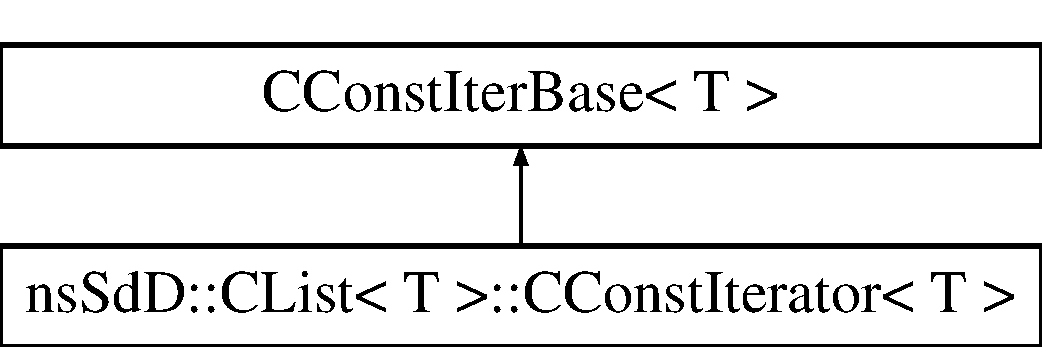
\includegraphics[height=2.000000cm]{structnsSdD_1_1CList_1_1CConstIterator}
\end{center}
\end{figure}
\subsection*{Public Member Functions}
\begin{DoxyCompactItemize}
\item 
\hyperlink{structnsSdD_1_1CList_1_1CConstIterator_a2a5d916c0ecc7397ade18c0e612f8b8a}{C\+Const\+Iterator} (C\+Node\+Ptr p=nullptr) noexcept
\begin{DoxyCompactList}\small\item\em The default constructor of the const\+\_\+iterator for the \hyperlink{classnsSdD_1_1CList}{C\+List} class. \end{DoxyCompactList}\item 
\hypertarget{structnsSdD_1_1CList_1_1CConstIterator_a4f1976b5f8708e35f927e946905a16d5}{\hyperlink{structnsSdD_1_1CList_1_1CConstIterator_a4f1976b5f8708e35f927e946905a16d5}{C\+Const\+Iterator} (const \hyperlink{structnsSdD_1_1CList_1_1CConstIterator}{C\+Const\+Iterator} \&)=default}\label{structnsSdD_1_1CList_1_1CConstIterator_a4f1976b5f8708e35f927e946905a16d5}

\begin{DoxyCompactList}\small\item\em The copy-\/constructor for the const\+\_\+iterator. \end{DoxyCompactList}\item 
\hyperlink{structnsSdD_1_1CList_1_1CConstIterator}{C\+Const\+Iterator} \& \hyperlink{structnsSdD_1_1CList_1_1CConstIterator_a5bcf62e3feee5725386ec2fd74ad9f7a}{operator=} (const \hyperlink{structnsSdD_1_1CList_1_1CConstIterator}{C\+Const\+Iterator} \&) noexcept=default
\begin{DoxyCompactList}\small\item\em The default operator= for the iterator. \end{DoxyCompactList}\item 
bool \hyperlink{structnsSdD_1_1CList_1_1CConstIterator_a00009d64b32bb3b29f95629d87289749}{operator==} (const \hyperlink{structnsSdD_1_1CList_1_1CConstIterator}{C\+Const\+Iterator} \&other) const noexcept
\begin{DoxyCompactList}\small\item\em The operator == who compare the two node and return true if equal and false otherwise. \end{DoxyCompactList}\item 
bool \hyperlink{structnsSdD_1_1CList_1_1CConstIterator_a11e78574976270f6360da8df191530a7}{operator!=} (const \hyperlink{structnsSdD_1_1CList_1_1CConstIterator}{C\+Const\+Iterator} \&other) const noexcept
\begin{DoxyCompactList}\small\item\em The operator != who compare the two node and return true if not equal and false otherwise. \end{DoxyCompactList}\item 
\hyperlink{structnsSdD_1_1CList_1_1CConstIterator}{C\+Const\+Iterator} \& \hyperlink{structnsSdD_1_1CList_1_1CConstIterator_a307985e2d8e6dc496d366de8a3ca624a}{operator++} () noexcept
\begin{DoxyCompactList}\small\item\em The operator ++ who pre-\/increment the iterator, pass to the next node. \end{DoxyCompactList}\item 
\hyperlink{structnsSdD_1_1CList_1_1CConstIterator}{C\+Const\+Iterator} \& \hyperlink{structnsSdD_1_1CList_1_1CConstIterator_af9d0e9415ed4b6a5735feb22e421ef69}{operator-\/-\/} () noexcept
\begin{DoxyCompactList}\small\item\em The operator -- who pre-\/decrement the iterator, pass to the previous node. \end{DoxyCompactList}\item 
\hyperlink{structnsSdD_1_1CList_1_1CConstIterator}{C\+Const\+Iterator} \hyperlink{structnsSdD_1_1CList_1_1CConstIterator_af63bd9514ce47807312698ac92a6cfec}{operator++} (int) noexcept
\begin{DoxyCompactList}\small\item\em The operator ++ who post-\/increment the iterator, pass to the next node. \end{DoxyCompactList}\item 
\hyperlink{structnsSdD_1_1CList_1_1CConstIterator}{C\+Const\+Iterator} \hyperlink{structnsSdD_1_1CList_1_1CConstIterator_a66443d7e5935d1b9703f477d49f2cdc8}{operator-\/-\/} (int) noexcept
\begin{DoxyCompactList}\small\item\em The operator -- who post-\/decrement the iterator, pass to the previous node. \end{DoxyCompactList}\item 
C\+Const\+Iter\+Base$<$ T $>$\+::pointer \hyperlink{structnsSdD_1_1CList_1_1CConstIterator_aee6015666c2eea5b396f1b1800b9b41d}{operator-\/$>$} () const noexcept
\begin{DoxyCompactList}\small\item\em The dereferencement operator -\/$>$ who return the a pointer to the info of the node. \end{DoxyCompactList}\item 
C\+Const\+Iter\+Base$<$ T $>$\+::reference \hyperlink{structnsSdD_1_1CList_1_1CConstIterator_a9c3bac52765a92e2ab2e964bf5df5e72}{operator$\ast$} () const noexcept
\begin{DoxyCompactList}\small\item\em The dereferencement operator $\ast$ who return the a reference to the info of the node. \end{DoxyCompactList}\item 
C\+Node\+Ptr \hyperlink{structnsSdD_1_1CList_1_1CConstIterator_a856f2ce0a4334188f7f5131159b24143}{get\+Node} () const noexcept
\begin{DoxyCompactList}\small\item\em The function return the node of the pointer. \end{DoxyCompactList}\end{DoxyCompactItemize}


\subsection{Constructor \& Destructor Documentation}
\hypertarget{structnsSdD_1_1CList_1_1CConstIterator_a2a5d916c0ecc7397ade18c0e612f8b8a}{\index{ns\+Sd\+D\+::\+C\+List\+::\+C\+Const\+Iterator@{ns\+Sd\+D\+::\+C\+List\+::\+C\+Const\+Iterator}!C\+Const\+Iterator@{C\+Const\+Iterator}}
\index{C\+Const\+Iterator@{C\+Const\+Iterator}!ns\+Sd\+D\+::\+C\+List\+::\+C\+Const\+Iterator@{ns\+Sd\+D\+::\+C\+List\+::\+C\+Const\+Iterator}}
\subsubsection[{C\+Const\+Iterator}]{\setlength{\rightskip}{0pt plus 5cm}template$<$typename T$>$ template$<$typename T $>$ {\bf ns\+Sd\+D\+::\+C\+List}$<$ T $>$\+::{\bf C\+Const\+Iterator}$<$ T $>$\+::{\bf C\+Const\+Iterator} (
\begin{DoxyParamCaption}
\item[{C\+Node\+Ptr}]{p = {\ttfamily nullptr}}
\end{DoxyParamCaption}
)\hspace{0.3cm}{\ttfamily [inline]}, {\ttfamily [noexcept]}}}\label{structnsSdD_1_1CList_1_1CConstIterator_a2a5d916c0ecc7397ade18c0e612f8b8a}


The default constructor of the const\+\_\+iterator for the \hyperlink{classnsSdD_1_1CList}{C\+List} class. 


\begin{DoxyParams}[1]{Parameters}
\mbox{\tt in}  & {\em p} & The the node we want to use to construct the iterator. \\
\hline
\end{DoxyParams}


\subsection{Member Function Documentation}
\hypertarget{structnsSdD_1_1CList_1_1CConstIterator_a856f2ce0a4334188f7f5131159b24143}{\index{ns\+Sd\+D\+::\+C\+List\+::\+C\+Const\+Iterator@{ns\+Sd\+D\+::\+C\+List\+::\+C\+Const\+Iterator}!get\+Node@{get\+Node}}
\index{get\+Node@{get\+Node}!ns\+Sd\+D\+::\+C\+List\+::\+C\+Const\+Iterator@{ns\+Sd\+D\+::\+C\+List\+::\+C\+Const\+Iterator}}
\subsubsection[{get\+Node}]{\setlength{\rightskip}{0pt plus 5cm}template$<$typename T$>$ template$<$typename T $>$ {\bf ns\+Sd\+D\+::\+C\+List}$<$ T $>$\+::{\bf C\+Const\+Iterator}$<$ T $>$\+::get\+Node (
\begin{DoxyParamCaption}
{}
\end{DoxyParamCaption}
) const\hspace{0.3cm}{\ttfamily [inline]}, {\ttfamily [noexcept]}}}\label{structnsSdD_1_1CList_1_1CConstIterator_a856f2ce0a4334188f7f5131159b24143}


The function return the node of the pointer. 

\begin{DoxyReturn}{Returns}
C\+Node\+Ptr The node of the pointer. 
\end{DoxyReturn}
\hypertarget{structnsSdD_1_1CList_1_1CConstIterator_a11e78574976270f6360da8df191530a7}{\index{ns\+Sd\+D\+::\+C\+List\+::\+C\+Const\+Iterator@{ns\+Sd\+D\+::\+C\+List\+::\+C\+Const\+Iterator}!operator"!=@{operator"!=}}
\index{operator"!=@{operator"!=}!ns\+Sd\+D\+::\+C\+List\+::\+C\+Const\+Iterator@{ns\+Sd\+D\+::\+C\+List\+::\+C\+Const\+Iterator}}
\subsubsection[{operator"!=}]{\setlength{\rightskip}{0pt plus 5cm}template$<$typename T$>$ template$<$typename T $>$ {\bf ns\+Sd\+D\+::\+C\+List}$<$ T $>$\+::{\bf C\+Const\+Iterator}$<$ T $>$\+::operator!= (
\begin{DoxyParamCaption}
\item[{const {\bf C\+Const\+Iterator}$<$ T $>$ \&}]{other}
\end{DoxyParamCaption}
) const\hspace{0.3cm}{\ttfamily [inline]}, {\ttfamily [noexcept]}}}\label{structnsSdD_1_1CList_1_1CConstIterator_a11e78574976270f6360da8df191530a7}


The operator != who compare the two node and return true if not equal and false otherwise. 


\begin{DoxyParams}[1]{Parameters}
\mbox{\tt in}  & {\em other} & The value we want to compare. \\
\hline
\end{DoxyParams}
\begin{DoxyReturn}{Returns}
bool If the two iterator are not equal. 
\end{DoxyReturn}
\hypertarget{structnsSdD_1_1CList_1_1CConstIterator_a9c3bac52765a92e2ab2e964bf5df5e72}{\index{ns\+Sd\+D\+::\+C\+List\+::\+C\+Const\+Iterator@{ns\+Sd\+D\+::\+C\+List\+::\+C\+Const\+Iterator}!operator$\ast$@{operator$\ast$}}
\index{operator$\ast$@{operator$\ast$}!ns\+Sd\+D\+::\+C\+List\+::\+C\+Const\+Iterator@{ns\+Sd\+D\+::\+C\+List\+::\+C\+Const\+Iterator}}
\subsubsection[{operator$\ast$}]{\setlength{\rightskip}{0pt plus 5cm}template$<$typename T$>$ template$<$typename T $>$ {\bf ns\+Sd\+D\+::\+C\+List}$<$ T $>$\+::{\bf C\+Const\+Iterator}$<$ T $>$\+::operator$\ast$ (
\begin{DoxyParamCaption}
{}
\end{DoxyParamCaption}
) const\hspace{0.3cm}{\ttfamily [inline]}, {\ttfamily [noexcept]}}}\label{structnsSdD_1_1CList_1_1CConstIterator_a9c3bac52765a92e2ab2e964bf5df5e72}


The dereferencement operator $\ast$ who return the a reference to the info of the node. 

\begin{DoxyReturn}{Returns}
C\+Iter\+Base$<$\+T$>$\+::reference The reference to the value of the node. 
\end{DoxyReturn}
\hypertarget{structnsSdD_1_1CList_1_1CConstIterator_a307985e2d8e6dc496d366de8a3ca624a}{\index{ns\+Sd\+D\+::\+C\+List\+::\+C\+Const\+Iterator@{ns\+Sd\+D\+::\+C\+List\+::\+C\+Const\+Iterator}!operator++@{operator++}}
\index{operator++@{operator++}!ns\+Sd\+D\+::\+C\+List\+::\+C\+Const\+Iterator@{ns\+Sd\+D\+::\+C\+List\+::\+C\+Const\+Iterator}}
\subsubsection[{operator++}]{\setlength{\rightskip}{0pt plus 5cm}template$<$typename T$>$ template$<$typename T $>$ {\bf ns\+Sd\+D\+::\+C\+List}$<$ T $>$\+::{\bf C\+Const\+Iterator}$<$ T $>$\+::operator++ (
\begin{DoxyParamCaption}
{}
\end{DoxyParamCaption}
)\hspace{0.3cm}{\ttfamily [inline]}, {\ttfamily [noexcept]}}}\label{structnsSdD_1_1CList_1_1CConstIterator_a307985e2d8e6dc496d366de8a3ca624a}


The operator ++ who pre-\/increment the iterator, pass to the next node. 

\begin{DoxyReturn}{Returns}
C\+Constterator The iterator with the new value. 
\end{DoxyReturn}
\hypertarget{structnsSdD_1_1CList_1_1CConstIterator_af63bd9514ce47807312698ac92a6cfec}{\index{ns\+Sd\+D\+::\+C\+List\+::\+C\+Const\+Iterator@{ns\+Sd\+D\+::\+C\+List\+::\+C\+Const\+Iterator}!operator++@{operator++}}
\index{operator++@{operator++}!ns\+Sd\+D\+::\+C\+List\+::\+C\+Const\+Iterator@{ns\+Sd\+D\+::\+C\+List\+::\+C\+Const\+Iterator}}
\subsubsection[{operator++}]{\setlength{\rightskip}{0pt plus 5cm}template$<$typename T$>$ template$<$typename T $>$ {\bf ns\+Sd\+D\+::\+C\+List}$<$ T $>$\+::{\bf C\+Const\+Iterator}$<$ T $>$\+::operator++ (
\begin{DoxyParamCaption}
\item[{int}]{}
\end{DoxyParamCaption}
)\hspace{0.3cm}{\ttfamily [inline]}, {\ttfamily [noexcept]}}}\label{structnsSdD_1_1CList_1_1CConstIterator_af63bd9514ce47807312698ac92a6cfec}


The operator ++ who post-\/increment the iterator, pass to the next node. 

\begin{DoxyReturn}{Returns}
C\+Const\+C\+Iterator The iterator with the old value, but iterator are increment. 
\end{DoxyReturn}
\hypertarget{structnsSdD_1_1CList_1_1CConstIterator_af9d0e9415ed4b6a5735feb22e421ef69}{\index{ns\+Sd\+D\+::\+C\+List\+::\+C\+Const\+Iterator@{ns\+Sd\+D\+::\+C\+List\+::\+C\+Const\+Iterator}!operator-\/-\/@{operator-\/-\/}}
\index{operator-\/-\/@{operator-\/-\/}!ns\+Sd\+D\+::\+C\+List\+::\+C\+Const\+Iterator@{ns\+Sd\+D\+::\+C\+List\+::\+C\+Const\+Iterator}}
\subsubsection[{operator-\/-\/}]{\setlength{\rightskip}{0pt plus 5cm}template$<$typename T$>$ template$<$typename T $>$ {\bf ns\+Sd\+D\+::\+C\+List}$<$ T $>$\+::{\bf C\+Const\+Iterator}$<$ T $>$\+::operator-\/-\/ (
\begin{DoxyParamCaption}
{}
\end{DoxyParamCaption}
)\hspace{0.3cm}{\ttfamily [inline]}, {\ttfamily [noexcept]}}}\label{structnsSdD_1_1CList_1_1CConstIterator_af9d0e9415ed4b6a5735feb22e421ef69}


The operator -- who pre-\/decrement the iterator, pass to the previous node. 

\begin{DoxyReturn}{Returns}
C\+Constterator The iterator with the new value. 
\end{DoxyReturn}
\hypertarget{structnsSdD_1_1CList_1_1CConstIterator_a66443d7e5935d1b9703f477d49f2cdc8}{\index{ns\+Sd\+D\+::\+C\+List\+::\+C\+Const\+Iterator@{ns\+Sd\+D\+::\+C\+List\+::\+C\+Const\+Iterator}!operator-\/-\/@{operator-\/-\/}}
\index{operator-\/-\/@{operator-\/-\/}!ns\+Sd\+D\+::\+C\+List\+::\+C\+Const\+Iterator@{ns\+Sd\+D\+::\+C\+List\+::\+C\+Const\+Iterator}}
\subsubsection[{operator-\/-\/}]{\setlength{\rightskip}{0pt plus 5cm}template$<$typename T$>$ template$<$typename T $>$ {\bf ns\+Sd\+D\+::\+C\+List}$<$ T $>$\+::{\bf C\+Const\+Iterator}$<$ T $>$\+::operator-\/-\/ (
\begin{DoxyParamCaption}
\item[{int}]{}
\end{DoxyParamCaption}
)\hspace{0.3cm}{\ttfamily [inline]}, {\ttfamily [noexcept]}}}\label{structnsSdD_1_1CList_1_1CConstIterator_a66443d7e5935d1b9703f477d49f2cdc8}


The operator -- who post-\/decrement the iterator, pass to the previous node. 

\begin{DoxyReturn}{Returns}
C\+Constterator The iterator with the old value, but iterator are decrement. 
\end{DoxyReturn}
\hypertarget{structnsSdD_1_1CList_1_1CConstIterator_aee6015666c2eea5b396f1b1800b9b41d}{\index{ns\+Sd\+D\+::\+C\+List\+::\+C\+Const\+Iterator@{ns\+Sd\+D\+::\+C\+List\+::\+C\+Const\+Iterator}!operator-\/$>$@{operator-\/$>$}}
\index{operator-\/$>$@{operator-\/$>$}!ns\+Sd\+D\+::\+C\+List\+::\+C\+Const\+Iterator@{ns\+Sd\+D\+::\+C\+List\+::\+C\+Const\+Iterator}}
\subsubsection[{operator-\/$>$}]{\setlength{\rightskip}{0pt plus 5cm}template$<$typename T$>$ template$<$typename T $>$ {\bf ns\+Sd\+D\+::\+C\+List}$<$ T $>$\+::{\bf C\+Const\+Iterator}$<$ T $>$\+::operator-\/$>$ (
\begin{DoxyParamCaption}
{}
\end{DoxyParamCaption}
) const\hspace{0.3cm}{\ttfamily [inline]}, {\ttfamily [noexcept]}}}\label{structnsSdD_1_1CList_1_1CConstIterator_aee6015666c2eea5b396f1b1800b9b41d}


The dereferencement operator -\/$>$ who return the a pointer to the info of the node. 

\begin{DoxyReturn}{Returns}
C\+Iter\+Base$<$\+T$>$\+::pointer The pointer to the value of the node. 
\end{DoxyReturn}
\hypertarget{structnsSdD_1_1CList_1_1CConstIterator_a5bcf62e3feee5725386ec2fd74ad9f7a}{\index{ns\+Sd\+D\+::\+C\+List\+::\+C\+Const\+Iterator@{ns\+Sd\+D\+::\+C\+List\+::\+C\+Const\+Iterator}!operator=@{operator=}}
\index{operator=@{operator=}!ns\+Sd\+D\+::\+C\+List\+::\+C\+Const\+Iterator@{ns\+Sd\+D\+::\+C\+List\+::\+C\+Const\+Iterator}}
\subsubsection[{operator=}]{\setlength{\rightskip}{0pt plus 5cm}template$<$typename T$>$ template$<$typename T $>$ {\bf ns\+Sd\+D\+::\+C\+List}$<$ T $>$\+::{\bf C\+Const\+Iterator}$<$ T $>$\+::operator= (
\begin{DoxyParamCaption}
\item[{const {\bf C\+Const\+Iterator}$<$ T $>$ \&}]{}
\end{DoxyParamCaption}
)\hspace{0.3cm}{\ttfamily [default]}, {\ttfamily [noexcept]}}}\label{structnsSdD_1_1CList_1_1CConstIterator_a5bcf62e3feee5725386ec2fd74ad9f7a}


The default operator= for the iterator. 

\begin{DoxyReturn}{Returns}
\hyperlink{structnsSdD_1_1CList_1_1CConstIterator}{C\+Const\+Iterator} The new value of the const\+\_\+iterator. 
\end{DoxyReturn}
\hypertarget{structnsSdD_1_1CList_1_1CConstIterator_a00009d64b32bb3b29f95629d87289749}{\index{ns\+Sd\+D\+::\+C\+List\+::\+C\+Const\+Iterator@{ns\+Sd\+D\+::\+C\+List\+::\+C\+Const\+Iterator}!operator==@{operator==}}
\index{operator==@{operator==}!ns\+Sd\+D\+::\+C\+List\+::\+C\+Const\+Iterator@{ns\+Sd\+D\+::\+C\+List\+::\+C\+Const\+Iterator}}
\subsubsection[{operator==}]{\setlength{\rightskip}{0pt plus 5cm}template$<$typename T$>$ template$<$typename T $>$ {\bf ns\+Sd\+D\+::\+C\+List}$<$ T $>$\+::{\bf C\+Const\+Iterator}$<$ T $>$\+::operator== (
\begin{DoxyParamCaption}
\item[{const {\bf C\+Const\+Iterator}$<$ T $>$ \&}]{other}
\end{DoxyParamCaption}
) const\hspace{0.3cm}{\ttfamily [inline]}, {\ttfamily [noexcept]}}}\label{structnsSdD_1_1CList_1_1CConstIterator_a00009d64b32bb3b29f95629d87289749}


The operator == who compare the two node and return true if equal and false otherwise. 


\begin{DoxyParams}[1]{Parameters}
\mbox{\tt in}  & {\em other} & The value we want to compare. \\
\hline
\end{DoxyParams}
\begin{DoxyReturn}{Returns}
bool If the two iterator are equal. 
\end{DoxyReturn}


The documentation for this struct was generated from the following file\+:\begin{DoxyCompactItemize}
\item 
\hyperlink{CConstIterator_8hxx}{C\+Const\+Iterator.\+hxx}\end{DoxyCompactItemize}

\hypertarget{structnsSdD_1_1CList_1_1CIterator}{\section{ns\+Sd\+D\+:\+:C\+List$<$ T $>$\+:\+:C\+Iterator$<$ T $>$ Struct Template Reference}
\label{structnsSdD_1_1CList_1_1CIterator}\index{ns\+Sd\+D\+::\+C\+List$<$ T $>$\+::\+C\+Iterator$<$ T $>$@{ns\+Sd\+D\+::\+C\+List$<$ T $>$\+::\+C\+Iterator$<$ T $>$}}
}


This class is a personnal implementation of iterator for our class \hyperlink{classnsSdD_1_1CList}{C\+List}. We provide the essential function to work with us. We implement bidirectionnal iterator because we choose to use a double-\/linked list.  




{\ttfamily \#include $<$C\+Iterator.\+hxx$>$}

Inheritance diagram for ns\+Sd\+D\+:\+:C\+List$<$ T $>$\+:\+:C\+Iterator$<$ T $>$\+:\begin{figure}[H]
\begin{center}
\leavevmode
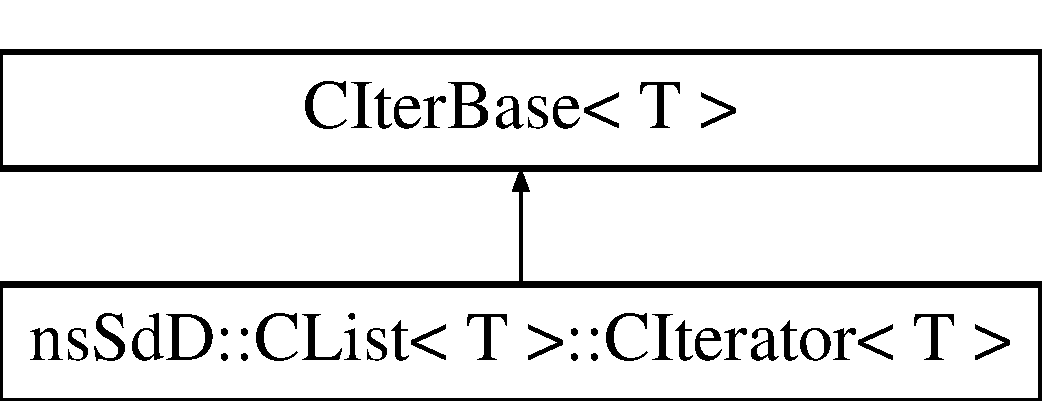
\includegraphics[height=2.000000cm]{structnsSdD_1_1CList_1_1CIterator}
\end{center}
\end{figure}
\subsection*{Public Member Functions}
\begin{DoxyCompactItemize}
\item 
\hyperlink{structnsSdD_1_1CList_1_1CIterator_a121a102242fccc875b9dfaceffbe9b07}{C\+Iterator} (C\+Node\+Ptr p=nullptr) noexcept
\begin{DoxyCompactList}\small\item\em The default constructor of the iterator for the \hyperlink{classnsSdD_1_1CList}{C\+List} class. \end{DoxyCompactList}\item 
\hypertarget{structnsSdD_1_1CList_1_1CIterator_aecc67a49d5805151e8f961ff8c6f5f39}{\hyperlink{structnsSdD_1_1CList_1_1CIterator_aecc67a49d5805151e8f961ff8c6f5f39}{C\+Iterator} (const \hyperlink{structnsSdD_1_1CList_1_1CIterator}{C\+Iterator} \&) noexcept=default}\label{structnsSdD_1_1CList_1_1CIterator_aecc67a49d5805151e8f961ff8c6f5f39}

\begin{DoxyCompactList}\small\item\em The copy-\/constructor for the iterator. \end{DoxyCompactList}\item 
\hypertarget{structnsSdD_1_1CList_1_1CIterator_a222bd54da7e51ca4a6aa82ebc7264ba1}{\hyperlink{structnsSdD_1_1CList_1_1CIterator}{C\+Iterator} \& \hyperlink{structnsSdD_1_1CList_1_1CIterator_a222bd54da7e51ca4a6aa82ebc7264ba1}{operator=} (const \hyperlink{structnsSdD_1_1CList_1_1CIterator}{C\+Iterator} \&) noexcept=default}\label{structnsSdD_1_1CList_1_1CIterator_a222bd54da7e51ca4a6aa82ebc7264ba1}

\begin{DoxyCompactList}\small\item\em The default operator= for the iterator. \end{DoxyCompactList}\item 
\hyperlink{structnsSdD_1_1CList_1_1CIterator}{C\+Iterator} \& \hyperlink{structnsSdD_1_1CList_1_1CIterator_a3153cc52b78734144f0aceb2d6d315c3}{operator=} (const T \&info) noexcept
\begin{DoxyCompactList}\small\item\em The operator = to assign a value to the iterator. \end{DoxyCompactList}\item 
bool \hyperlink{structnsSdD_1_1CList_1_1CIterator_a16afbe0c358f1f88eb9eafe9093228d0}{operator==} (const \hyperlink{structnsSdD_1_1CList_1_1CIterator}{C\+Iterator} \&other) const noexcept
\begin{DoxyCompactList}\small\item\em The operator == who compare the two node and return true if equal and false otherwise. \end{DoxyCompactList}\item 
bool \hyperlink{structnsSdD_1_1CList_1_1CIterator_ade896f4a807e6c8ac4185b3c060f58f8}{operator!=} (const \hyperlink{structnsSdD_1_1CList_1_1CIterator}{C\+Iterator} \&other) const noexcept
\begin{DoxyCompactList}\small\item\em The operator != who compare the two node and return true if not equal and false otherwise. \end{DoxyCompactList}\item 
\hyperlink{structnsSdD_1_1CList_1_1CIterator}{C\+Iterator} \& \hyperlink{structnsSdD_1_1CList_1_1CIterator_a50bdb955c4141339f69853d59d61f838}{operator++} () noexcept
\begin{DoxyCompactList}\small\item\em The operator ++ who pre-\/increment the iterator, pass to the next node. \end{DoxyCompactList}\item 
\hyperlink{structnsSdD_1_1CList_1_1CIterator}{C\+Iterator} \& \hyperlink{structnsSdD_1_1CList_1_1CIterator_af0398db8fae3641ab46fe3d8806cd185}{operator-\/-\/} () noexcept
\begin{DoxyCompactList}\small\item\em The operator -- who pre-\/decrement the iterator, pass to the previous node. \end{DoxyCompactList}\item 
\hyperlink{structnsSdD_1_1CList_1_1CIterator}{C\+Iterator} \hyperlink{structnsSdD_1_1CList_1_1CIterator_a8304ea60a13fc7818d943241934e8169}{operator++} (int) noexcept
\begin{DoxyCompactList}\small\item\em The operator ++ who post-\/increment the iterator, pass to the next node. \end{DoxyCompactList}\item 
\hyperlink{structnsSdD_1_1CList_1_1CIterator}{C\+Iterator} \hyperlink{structnsSdD_1_1CList_1_1CIterator_a3a74d1ce68a46e0d9d63130b5340a09b}{operator-\/-\/} (int) noexcept
\begin{DoxyCompactList}\small\item\em The operator -- who post-\/decrement the iterator, pass to the previous node. \end{DoxyCompactList}\item 
C\+Iter\+Base$<$ T $>$\+::pointer \hyperlink{structnsSdD_1_1CList_1_1CIterator_a36b69ff32014bb4669c18c8da9e10d65}{operator-\/$>$} () noexcept
\begin{DoxyCompactList}\small\item\em The dereferencement operator -\/$>$ who return the a pointer to the info of the node. \end{DoxyCompactList}\item 
C\+Iter\+Base$<$ T $>$\+::reference \hyperlink{structnsSdD_1_1CList_1_1CIterator_aecbfd6f490eb99c310ef9b57b8df9ea6}{operator$\ast$} () noexcept
\begin{DoxyCompactList}\small\item\em The dereferencement operator $\ast$ who return the a reference to the info of the node. \end{DoxyCompactList}\item 
C\+Iter\+Base$<$ T $>$\+::reference \hyperlink{structnsSdD_1_1CList_1_1CIterator_aa9995f10a811b8d3c49f9799a8d42170}{operator$\ast$} () const noexcept
\begin{DoxyCompactList}\small\item\em The dereferencement operator $\ast$ who return the a reference to the info of the node. \end{DoxyCompactList}\item 
C\+Node\+Ptr \hyperlink{structnsSdD_1_1CList_1_1CIterator_a9c99745d084ce7e1fa1b304fd527e9e7}{get\+Node} () const noexcept
\begin{DoxyCompactList}\small\item\em The function return the node of the pointer. \end{DoxyCompactList}\end{DoxyCompactItemize}


\subsection{Detailed Description}
\subsubsection*{template$<$typename T$>$template$<$typename T$>$struct ns\+Sd\+D\+::\+C\+List$<$ T $>$\+::\+C\+Iterator$<$ T $>$}

This class is a personnal implementation of iterator for our class \hyperlink{classnsSdD_1_1CList}{C\+List}. We provide the essential function to work with us. We implement bidirectionnal iterator because we choose to use a double-\/linked list. 

\subsection{Constructor \& Destructor Documentation}
\hypertarget{structnsSdD_1_1CList_1_1CIterator_a121a102242fccc875b9dfaceffbe9b07}{\index{ns\+Sd\+D\+::\+C\+List\+::\+C\+Iterator@{ns\+Sd\+D\+::\+C\+List\+::\+C\+Iterator}!C\+Iterator@{C\+Iterator}}
\index{C\+Iterator@{C\+Iterator}!ns\+Sd\+D\+::\+C\+List\+::\+C\+Iterator@{ns\+Sd\+D\+::\+C\+List\+::\+C\+Iterator}}
\subsubsection[{C\+Iterator}]{\setlength{\rightskip}{0pt plus 5cm}template$<$typename T$>$ template$<$typename T $>$ {\bf ns\+Sd\+D\+::\+C\+List}$<$ T $>$\+::{\bf C\+Iterator}$<$ T $>$\+::{\bf C\+Iterator} (
\begin{DoxyParamCaption}
\item[{C\+Node\+Ptr}]{p = {\ttfamily nullptr}}
\end{DoxyParamCaption}
)\hspace{0.3cm}{\ttfamily [inline]}, {\ttfamily [noexcept]}}}\label{structnsSdD_1_1CList_1_1CIterator_a121a102242fccc875b9dfaceffbe9b07}


The default constructor of the iterator for the \hyperlink{classnsSdD_1_1CList}{C\+List} class. 


\begin{DoxyParams}[1]{Parameters}
\mbox{\tt in}  & {\em p} & The the node we want to use to construct the iterator. \\
\hline
\end{DoxyParams}


\subsection{Member Function Documentation}
\hypertarget{structnsSdD_1_1CList_1_1CIterator_a9c99745d084ce7e1fa1b304fd527e9e7}{\index{ns\+Sd\+D\+::\+C\+List\+::\+C\+Iterator@{ns\+Sd\+D\+::\+C\+List\+::\+C\+Iterator}!get\+Node@{get\+Node}}
\index{get\+Node@{get\+Node}!ns\+Sd\+D\+::\+C\+List\+::\+C\+Iterator@{ns\+Sd\+D\+::\+C\+List\+::\+C\+Iterator}}
\subsubsection[{get\+Node}]{\setlength{\rightskip}{0pt plus 5cm}template$<$typename T$>$ template$<$typename T $>$ {\bf ns\+Sd\+D\+::\+C\+List}$<$ T $>$\+::{\bf C\+Iterator}$<$ T $>$\+::get\+Node (
\begin{DoxyParamCaption}
{}
\end{DoxyParamCaption}
) const\hspace{0.3cm}{\ttfamily [inline]}, {\ttfamily [noexcept]}}}\label{structnsSdD_1_1CList_1_1CIterator_a9c99745d084ce7e1fa1b304fd527e9e7}


The function return the node of the pointer. 

\begin{DoxyReturn}{Returns}
C\+Node\+Ptr The node of the pointer. 
\end{DoxyReturn}
\hypertarget{structnsSdD_1_1CList_1_1CIterator_ade896f4a807e6c8ac4185b3c060f58f8}{\index{ns\+Sd\+D\+::\+C\+List\+::\+C\+Iterator@{ns\+Sd\+D\+::\+C\+List\+::\+C\+Iterator}!operator"!=@{operator"!=}}
\index{operator"!=@{operator"!=}!ns\+Sd\+D\+::\+C\+List\+::\+C\+Iterator@{ns\+Sd\+D\+::\+C\+List\+::\+C\+Iterator}}
\subsubsection[{operator"!=}]{\setlength{\rightskip}{0pt plus 5cm}template$<$typename T$>$ template$<$typename T $>$ {\bf ns\+Sd\+D\+::\+C\+List}$<$ T $>$\+::{\bf C\+Iterator}$<$ T $>$\+::operator!= (
\begin{DoxyParamCaption}
\item[{const {\bf C\+Iterator}$<$ T $>$ \&}]{other}
\end{DoxyParamCaption}
) const\hspace{0.3cm}{\ttfamily [inline]}, {\ttfamily [noexcept]}}}\label{structnsSdD_1_1CList_1_1CIterator_ade896f4a807e6c8ac4185b3c060f58f8}


The operator != who compare the two node and return true if not equal and false otherwise. 


\begin{DoxyParams}[1]{Parameters}
\mbox{\tt in}  & {\em other} & The value we want to compare. \\
\hline
\end{DoxyParams}
\begin{DoxyReturn}{Returns}
bool If the two iterator are not equal. 
\end{DoxyReturn}
\hypertarget{structnsSdD_1_1CList_1_1CIterator_aecbfd6f490eb99c310ef9b57b8df9ea6}{\index{ns\+Sd\+D\+::\+C\+List\+::\+C\+Iterator@{ns\+Sd\+D\+::\+C\+List\+::\+C\+Iterator}!operator$\ast$@{operator$\ast$}}
\index{operator$\ast$@{operator$\ast$}!ns\+Sd\+D\+::\+C\+List\+::\+C\+Iterator@{ns\+Sd\+D\+::\+C\+List\+::\+C\+Iterator}}
\subsubsection[{operator$\ast$}]{\setlength{\rightskip}{0pt plus 5cm}template$<$typename T$>$ template$<$typename T $>$ {\bf ns\+Sd\+D\+::\+C\+List}$<$ T $>$\+::{\bf C\+Iterator}$<$ T $>$\+::operator$\ast$ (
\begin{DoxyParamCaption}
{}
\end{DoxyParamCaption}
)\hspace{0.3cm}{\ttfamily [inline]}, {\ttfamily [noexcept]}}}\label{structnsSdD_1_1CList_1_1CIterator_aecbfd6f490eb99c310ef9b57b8df9ea6}


The dereferencement operator $\ast$ who return the a reference to the info of the node. 

\begin{DoxyReturn}{Returns}
C\+Iter\+Base$<$\+T$>$\+::reference The reference to the value of the node. 
\end{DoxyReturn}
\hypertarget{structnsSdD_1_1CList_1_1CIterator_aa9995f10a811b8d3c49f9799a8d42170}{\index{ns\+Sd\+D\+::\+C\+List\+::\+C\+Iterator@{ns\+Sd\+D\+::\+C\+List\+::\+C\+Iterator}!operator$\ast$@{operator$\ast$}}
\index{operator$\ast$@{operator$\ast$}!ns\+Sd\+D\+::\+C\+List\+::\+C\+Iterator@{ns\+Sd\+D\+::\+C\+List\+::\+C\+Iterator}}
\subsubsection[{operator$\ast$}]{\setlength{\rightskip}{0pt plus 5cm}template$<$typename T$>$ template$<$typename T $>$ {\bf ns\+Sd\+D\+::\+C\+List}$<$ T $>$\+::{\bf C\+Iterator}$<$ T $>$\+::operator$\ast$ (
\begin{DoxyParamCaption}
{}
\end{DoxyParamCaption}
) const\hspace{0.3cm}{\ttfamily [inline]}, {\ttfamily [noexcept]}}}\label{structnsSdD_1_1CList_1_1CIterator_aa9995f10a811b8d3c49f9799a8d42170}


The dereferencement operator $\ast$ who return the a reference to the info of the node. 

\begin{DoxyReturn}{Returns}
C\+Iter\+Base$<$\+T$>$\+::reference The reference to the value of the node. 
\end{DoxyReturn}
\hypertarget{structnsSdD_1_1CList_1_1CIterator_a50bdb955c4141339f69853d59d61f838}{\index{ns\+Sd\+D\+::\+C\+List\+::\+C\+Iterator@{ns\+Sd\+D\+::\+C\+List\+::\+C\+Iterator}!operator++@{operator++}}
\index{operator++@{operator++}!ns\+Sd\+D\+::\+C\+List\+::\+C\+Iterator@{ns\+Sd\+D\+::\+C\+List\+::\+C\+Iterator}}
\subsubsection[{operator++}]{\setlength{\rightskip}{0pt plus 5cm}template$<$typename T$>$ template$<$typename T $>$ {\bf ns\+Sd\+D\+::\+C\+List}$<$ T $>$\+::{\bf C\+Iterator}$<$ T $>$\+::operator++ (
\begin{DoxyParamCaption}
{}
\end{DoxyParamCaption}
)\hspace{0.3cm}{\ttfamily [inline]}, {\ttfamily [noexcept]}}}\label{structnsSdD_1_1CList_1_1CIterator_a50bdb955c4141339f69853d59d61f838}


The operator ++ who pre-\/increment the iterator, pass to the next node. 

\begin{DoxyReturn}{Returns}
\hyperlink{structnsSdD_1_1CList_1_1CIterator}{C\+Iterator} The iterator with the new value. 
\end{DoxyReturn}
\hypertarget{structnsSdD_1_1CList_1_1CIterator_a8304ea60a13fc7818d943241934e8169}{\index{ns\+Sd\+D\+::\+C\+List\+::\+C\+Iterator@{ns\+Sd\+D\+::\+C\+List\+::\+C\+Iterator}!operator++@{operator++}}
\index{operator++@{operator++}!ns\+Sd\+D\+::\+C\+List\+::\+C\+Iterator@{ns\+Sd\+D\+::\+C\+List\+::\+C\+Iterator}}
\subsubsection[{operator++}]{\setlength{\rightskip}{0pt plus 5cm}template$<$typename T$>$ template$<$typename T $>$ {\bf ns\+Sd\+D\+::\+C\+List}$<$ T $>$\+::{\bf C\+Iterator}$<$ T $>$\+::operator++ (
\begin{DoxyParamCaption}
\item[{int}]{}
\end{DoxyParamCaption}
)\hspace{0.3cm}{\ttfamily [inline]}, {\ttfamily [noexcept]}}}\label{structnsSdD_1_1CList_1_1CIterator_a8304ea60a13fc7818d943241934e8169}


The operator ++ who post-\/increment the iterator, pass to the next node. 

\begin{DoxyReturn}{Returns}
\hyperlink{structnsSdD_1_1CList_1_1CIterator}{C\+Iterator} The iterator with the old value, but iterator are increment. 
\end{DoxyReturn}
\hypertarget{structnsSdD_1_1CList_1_1CIterator_af0398db8fae3641ab46fe3d8806cd185}{\index{ns\+Sd\+D\+::\+C\+List\+::\+C\+Iterator@{ns\+Sd\+D\+::\+C\+List\+::\+C\+Iterator}!operator-\/-\/@{operator-\/-\/}}
\index{operator-\/-\/@{operator-\/-\/}!ns\+Sd\+D\+::\+C\+List\+::\+C\+Iterator@{ns\+Sd\+D\+::\+C\+List\+::\+C\+Iterator}}
\subsubsection[{operator-\/-\/}]{\setlength{\rightskip}{0pt plus 5cm}template$<$typename T$>$ template$<$typename T $>$ {\bf ns\+Sd\+D\+::\+C\+List}$<$ T $>$\+::{\bf C\+Iterator}$<$ T $>$\+::operator-\/-\/ (
\begin{DoxyParamCaption}
{}
\end{DoxyParamCaption}
)\hspace{0.3cm}{\ttfamily [inline]}, {\ttfamily [noexcept]}}}\label{structnsSdD_1_1CList_1_1CIterator_af0398db8fae3641ab46fe3d8806cd185}


The operator -- who pre-\/decrement the iterator, pass to the previous node. 

\begin{DoxyReturn}{Returns}
\hyperlink{structnsSdD_1_1CList_1_1CIterator}{C\+Iterator} The iterator with the new value. 
\end{DoxyReturn}
\hypertarget{structnsSdD_1_1CList_1_1CIterator_a3a74d1ce68a46e0d9d63130b5340a09b}{\index{ns\+Sd\+D\+::\+C\+List\+::\+C\+Iterator@{ns\+Sd\+D\+::\+C\+List\+::\+C\+Iterator}!operator-\/-\/@{operator-\/-\/}}
\index{operator-\/-\/@{operator-\/-\/}!ns\+Sd\+D\+::\+C\+List\+::\+C\+Iterator@{ns\+Sd\+D\+::\+C\+List\+::\+C\+Iterator}}
\subsubsection[{operator-\/-\/}]{\setlength{\rightskip}{0pt plus 5cm}template$<$typename T$>$ template$<$typename T $>$ {\bf ns\+Sd\+D\+::\+C\+List}$<$ T $>$\+::{\bf C\+Iterator}$<$ T $>$\+::operator-\/-\/ (
\begin{DoxyParamCaption}
\item[{int}]{}
\end{DoxyParamCaption}
)\hspace{0.3cm}{\ttfamily [inline]}, {\ttfamily [noexcept]}}}\label{structnsSdD_1_1CList_1_1CIterator_a3a74d1ce68a46e0d9d63130b5340a09b}


The operator -- who post-\/decrement the iterator, pass to the previous node. 

\begin{DoxyReturn}{Returns}
\hyperlink{structnsSdD_1_1CList_1_1CIterator}{C\+Iterator} The iterator with the old value, but iterator are decrement. 
\end{DoxyReturn}
\hypertarget{structnsSdD_1_1CList_1_1CIterator_a36b69ff32014bb4669c18c8da9e10d65}{\index{ns\+Sd\+D\+::\+C\+List\+::\+C\+Iterator@{ns\+Sd\+D\+::\+C\+List\+::\+C\+Iterator}!operator-\/$>$@{operator-\/$>$}}
\index{operator-\/$>$@{operator-\/$>$}!ns\+Sd\+D\+::\+C\+List\+::\+C\+Iterator@{ns\+Sd\+D\+::\+C\+List\+::\+C\+Iterator}}
\subsubsection[{operator-\/$>$}]{\setlength{\rightskip}{0pt plus 5cm}template$<$typename T$>$ template$<$typename T $>$ {\bf ns\+Sd\+D\+::\+C\+List}$<$ T $>$\+::{\bf C\+Iterator}$<$ T $>$\+::operator-\/$>$ (
\begin{DoxyParamCaption}
{}
\end{DoxyParamCaption}
)\hspace{0.3cm}{\ttfamily [inline]}, {\ttfamily [noexcept]}}}\label{structnsSdD_1_1CList_1_1CIterator_a36b69ff32014bb4669c18c8da9e10d65}


The dereferencement operator -\/$>$ who return the a pointer to the info of the node. 

\begin{DoxyReturn}{Returns}
C\+Iter\+Base$<$\+T$>$\+::pointer The pointer to the value of the node. 
\end{DoxyReturn}
\hypertarget{structnsSdD_1_1CList_1_1CIterator_a3153cc52b78734144f0aceb2d6d315c3}{\index{ns\+Sd\+D\+::\+C\+List\+::\+C\+Iterator@{ns\+Sd\+D\+::\+C\+List\+::\+C\+Iterator}!operator=@{operator=}}
\index{operator=@{operator=}!ns\+Sd\+D\+::\+C\+List\+::\+C\+Iterator@{ns\+Sd\+D\+::\+C\+List\+::\+C\+Iterator}}
\subsubsection[{operator=}]{\setlength{\rightskip}{0pt plus 5cm}template$<$typename T$>$ template$<$typename T $>$ {\bf ns\+Sd\+D\+::\+C\+List}$<$ T $>$\+::{\bf C\+Iterator}$<$ T $>$\+::operator= (
\begin{DoxyParamCaption}
\item[{const T \&}]{info}
\end{DoxyParamCaption}
)\hspace{0.3cm}{\ttfamily [inline]}, {\ttfamily [noexcept]}}}\label{structnsSdD_1_1CList_1_1CIterator_a3153cc52b78734144f0aceb2d6d315c3}


The operator = to assign a value to the iterator. 


\begin{DoxyParams}[1]{Parameters}
\mbox{\tt in}  & {\em info} & The value we want to affect. \\
\hline
\end{DoxyParams}
\begin{DoxyReturn}{Returns}
\hyperlink{structnsSdD_1_1CList_1_1CIterator}{C\+Iterator} The new value of the iterator. 
\end{DoxyReturn}
\hypertarget{structnsSdD_1_1CList_1_1CIterator_a16afbe0c358f1f88eb9eafe9093228d0}{\index{ns\+Sd\+D\+::\+C\+List\+::\+C\+Iterator@{ns\+Sd\+D\+::\+C\+List\+::\+C\+Iterator}!operator==@{operator==}}
\index{operator==@{operator==}!ns\+Sd\+D\+::\+C\+List\+::\+C\+Iterator@{ns\+Sd\+D\+::\+C\+List\+::\+C\+Iterator}}
\subsubsection[{operator==}]{\setlength{\rightskip}{0pt plus 5cm}template$<$typename T$>$ template$<$typename T $>$ {\bf ns\+Sd\+D\+::\+C\+List}$<$ T $>$\+::{\bf C\+Iterator}$<$ T $>$\+::operator== (
\begin{DoxyParamCaption}
\item[{const {\bf C\+Iterator}$<$ T $>$ \&}]{other}
\end{DoxyParamCaption}
) const\hspace{0.3cm}{\ttfamily [inline]}, {\ttfamily [noexcept]}}}\label{structnsSdD_1_1CList_1_1CIterator_a16afbe0c358f1f88eb9eafe9093228d0}


The operator == who compare the two node and return true if equal and false otherwise. 


\begin{DoxyParams}[1]{Parameters}
\mbox{\tt in}  & {\em other} & The value we want to compare. \\
\hline
\end{DoxyParams}
\begin{DoxyReturn}{Returns}
bool If the two iterator are equal. 
\end{DoxyReturn}


The documentation for this struct was generated from the following file\+:\begin{DoxyCompactItemize}
\item 
\hyperlink{CIterator_8hxx}{C\+Iterator.\+hxx}\end{DoxyCompactItemize}

\hypertarget{classnsSdD_1_1CList}{\section{ns\+Sd\+D\+:\+:C\+List$<$ T $>$ Class Template Reference}
\label{classnsSdD_1_1CList}\index{ns\+Sd\+D\+::\+C\+List$<$ T $>$@{ns\+Sd\+D\+::\+C\+List$<$ T $>$}}
}


\hyperlink{classnsSdD_1_1CList}{C\+List} is the main class of our work, it's develop in order to be the most close to the original std\+::list In this idea we choose to make a double-\/linked list, in that way we can use bidirectional iterator and have a stl compliant \hyperlink{classnsSdD_1_1CList}{C\+List}. During the development process we choose to work in T\+D\+D (Test Driven Development) in order to have the least bugs possible.  




{\ttfamily \#include $<$C\+List.\+h$>$}

\subsection*{Classes}
\begin{DoxyCompactItemize}
\item 
struct \hyperlink{structnsSdD_1_1CList_1_1CConstIterator}{C\+Const\+Iterator}
\item 
struct \hyperlink{structnsSdD_1_1CList_1_1CIterator}{C\+Iterator}
\begin{DoxyCompactList}\small\item\em This class is a personnal implementation of iterator for our class \hyperlink{classnsSdD_1_1CList}{C\+List}. We provide the essential function to work with us. We implement bidirectionnal iterator because we choose to use a double-\/linked list. \end{DoxyCompactList}\item 
class \hyperlink{classnsSdD_1_1CList_1_1CNode}{C\+Node}
\end{DoxyCompactItemize}
\subsection*{Public Types}
\begin{DoxyCompactItemize}
\item 
\hypertarget{classnsSdD_1_1CList_a91d4b6b8c89816da277ee27d32df5478}{typedef size\+\_\+t \hyperlink{classnsSdD_1_1CList_a91d4b6b8c89816da277ee27d32df5478}{size\+\_\+type}}\label{classnsSdD_1_1CList_a91d4b6b8c89816da277ee27d32df5478}

\begin{DoxyCompactList}\small\item\em This define a {\ttfamily size\+\_\+t}. We use it because it's a std\+::list standard. \end{DoxyCompactList}\item 
\hypertarget{classnsSdD_1_1CList_afdaca29586106fc15940d8529f4990f8}{typedef \hyperlink{structnsSdD_1_1CList_1_1CIterator}{C\+Iterator} \hyperlink{classnsSdD_1_1CList_afdaca29586106fc15940d8529f4990f8}{iterator}}\label{classnsSdD_1_1CList_afdaca29586106fc15940d8529f4990f8}

\begin{DoxyCompactList}\small\item\em This define a {\ttfamily \hyperlink{structnsSdD_1_1CList_1_1CIterator}{C\+Iterator}}. We use it to declare a \hyperlink{classnsSdD_1_1CList}{C\+List} iterator. \end{DoxyCompactList}\item 
\hypertarget{classnsSdD_1_1CList_ae323732a26e507146686556fb775767a}{typedef \hyperlink{structnsSdD_1_1CList_1_1CConstIterator}{C\+Const\+Iterator} \hyperlink{classnsSdD_1_1CList_ae323732a26e507146686556fb775767a}{const\+\_\+iterator}}\label{classnsSdD_1_1CList_ae323732a26e507146686556fb775767a}

\begin{DoxyCompactList}\small\item\em This define a {\ttfamily \hyperlink{structnsSdD_1_1CList_1_1CConstIterator}{C\+Const\+Iterator}}. We use it to declare a \hyperlink{classnsSdD_1_1CList}{C\+List} const iterator. \end{DoxyCompactList}\item 
\hypertarget{classnsSdD_1_1CList_a5582eb88a5f625ef426f534ea5556311}{typedef std\+::reverse\+\_\+iterator\\*
$<$ \hyperlink{classnsSdD_1_1CList_afdaca29586106fc15940d8529f4990f8}{iterator} $>$ \hyperlink{classnsSdD_1_1CList_a5582eb88a5f625ef426f534ea5556311}{reverse\+\_\+iterator}}\label{classnsSdD_1_1CList_a5582eb88a5f625ef426f534ea5556311}

\begin{DoxyCompactList}\small\item\em This define a {\ttfamily C\+Reverse\+Iterator}. We use it to declare a \hyperlink{classnsSdD_1_1CList}{C\+List} reverse\+\_\+iterator. \end{DoxyCompactList}\item 
\hypertarget{classnsSdD_1_1CList_a43f361676af43c355821d20da82ad401}{typedef std\+::reverse\+\_\+iterator\\*
$<$ \hyperlink{classnsSdD_1_1CList_ae323732a26e507146686556fb775767a}{const\+\_\+iterator} $>$ \hyperlink{classnsSdD_1_1CList_a43f361676af43c355821d20da82ad401}{const\+\_\+reverse\+\_\+iterator}}\label{classnsSdD_1_1CList_a43f361676af43c355821d20da82ad401}

\begin{DoxyCompactList}\small\item\em This define a {\ttfamily C\+Const\+Reverse\+Iterator}. We use it to declare a \hyperlink{classnsSdD_1_1CList}{C\+List} const reverse iterator. \end{DoxyCompactList}\end{DoxyCompactItemize}
\subsection*{Public Member Functions}
\begin{DoxyCompactItemize}
\item 
\hyperlink{classnsSdD_1_1CList_aad7088db9f8120c6e6c1a2f39022fa8f}{C\+List} (const \hyperlink{classnsSdD_1_1CList}{C\+List}$<$ T $>$ \&x) noexcept
\begin{DoxyCompactList}\small\item\em This is the copy-\/constructor of the class \hyperlink{classnsSdD_1_1CList}{C\+List}. \end{DoxyCompactList}\item 
\hyperlink{classnsSdD_1_1CList_ae319d81f9a81a4d4aa5427f013fe8dae}{C\+List} () noexcept
\begin{DoxyCompactList}\small\item\em This is the default of the class \hyperlink{classnsSdD_1_1CList}{C\+List}. \end{DoxyCompactList}\item 
\hyperlink{classnsSdD_1_1CList_a0dc3fc05ef1e765313814baf2be139c1}{C\+List} (size\+\_\+t n) noexcept
\begin{DoxyCompactList}\small\item\em This is the constructor by the size ({\ttfamily size\+\_\+t} n) \hyperlink{classnsSdD_1_1CList}{C\+List} we want. The constructor create a \hyperlink{classnsSdD_1_1CList}{C\+List} of n elements. \end{DoxyCompactList}\item 
\hyperlink{classnsSdD_1_1CList_a09fd13d9614defdb880fdab1ae0b33ca}{C\+List} (size\+\_\+t n, const T \&val) noexcept
\begin{DoxyCompactList}\small\item\em This is the constructor by the size ({\ttfamily size\+\_\+t} n) \hyperlink{classnsSdD_1_1CList}{C\+List} we want. The constructor create a \hyperlink{classnsSdD_1_1CList}{C\+List} of n elements with {\ttfamily T} val in each element. \end{DoxyCompactList}\item 
\hypertarget{classnsSdD_1_1CList_a6558a45c50021a28a54ea3e48fd1ed4b}{{\footnotesize template$<$class Input\+Iterator $>$ }\\{\bfseries C\+List} (Input\+Iterator first, Input\+Iterator last) noexcept}\label{classnsSdD_1_1CList_a6558a45c50021a28a54ea3e48fd1ed4b}

\item 
C\+Node\+Ptr \hyperlink{classnsSdD_1_1CList_ac196a16661fe4cba73b339a4e2fcfb73}{get\+Head} () const noexcept
\begin{DoxyCompactList}\small\item\em This function return the head of the \hyperlink{classnsSdD_1_1CList}{C\+List}. \end{DoxyCompactList}\item 
C\+Node\+Ptr \hyperlink{classnsSdD_1_1CList_a05c986208bf4f4a9ede4731df50ed8d0}{get\+Tail} () const noexcept
\begin{DoxyCompactList}\small\item\em This function return the tail of the \hyperlink{classnsSdD_1_1CList}{C\+List}. \end{DoxyCompactList}\item 
\hyperlink{structnsSdD_1_1CList_1_1CIterator}{C\+Iterator} \hyperlink{classnsSdD_1_1CList_aa388b52d241c12737c4e5b2a36c767c3}{begin} () noexcept
\begin{DoxyCompactList}\small\item\em This function construct and return A \hyperlink{structnsSdD_1_1CList_1_1CIterator}{C\+Iterator} to the begin of the \hyperlink{classnsSdD_1_1CList}{C\+List}. \end{DoxyCompactList}\item 
\hyperlink{structnsSdD_1_1CList_1_1CIterator}{C\+Iterator} \hyperlink{classnsSdD_1_1CList_ae1ed05415dfeb92174e030f9de754dc2}{end} () noexcept
\begin{DoxyCompactList}\small\item\em This function construct and return A \hyperlink{structnsSdD_1_1CList_1_1CIterator}{C\+Iterator} to the end of the \hyperlink{classnsSdD_1_1CList}{C\+List}. \end{DoxyCompactList}\item 
\hyperlink{structnsSdD_1_1CList_1_1CConstIterator}{C\+Const\+Iterator} \hyperlink{classnsSdD_1_1CList_a65cc2b6af1a489f45d2a3354c67fca39}{cbegin} () const noexcept
\begin{DoxyCompactList}\small\item\em This function construct and return a \hyperlink{structnsSdD_1_1CList_1_1CConstIterator}{C\+Const\+Iterator} to the begin of the \hyperlink{classnsSdD_1_1CList}{C\+List}. \end{DoxyCompactList}\item 
\hyperlink{structnsSdD_1_1CList_1_1CConstIterator}{C\+Const\+Iterator} \hyperlink{classnsSdD_1_1CList_a6fafea01ba64eb323ebe32e0eb6e6e6e}{cend} () const noexcept
\begin{DoxyCompactList}\small\item\em This function construct and return a \hyperlink{structnsSdD_1_1CList_1_1CIterator}{C\+Iterator} to the end of the \hyperlink{classnsSdD_1_1CList}{C\+List}. \end{DoxyCompactList}\item 
std\+::reverse\+\_\+iterator$<$ \hyperlink{structnsSdD_1_1CList_1_1CIterator}{C\+Iterator} $>$ \hyperlink{classnsSdD_1_1CList_a763731bf428359807d4c35f21ed1ac4e}{rbegin} () noexcept
\begin{DoxyCompactList}\small\item\em This function construct and return an reverse\+\_\+iterator to the end of the \hyperlink{classnsSdD_1_1CList}{C\+List}. \end{DoxyCompactList}\item 
std\+::reverse\+\_\+iterator$<$ \hyperlink{structnsSdD_1_1CList_1_1CIterator}{C\+Iterator} $>$ \hyperlink{classnsSdD_1_1CList_a971d1f0ea06ae04c61303705f05a4211}{rend} () noexcept
\begin{DoxyCompactList}\small\item\em This function construct and return an reverse\+\_\+iterator to the begin of the \hyperlink{classnsSdD_1_1CList}{C\+List}. \end{DoxyCompactList}\item 
std\+::reverse\+\_\+iterator\\*
$<$ \hyperlink{structnsSdD_1_1CList_1_1CConstIterator}{C\+Const\+Iterator} $>$ \hyperlink{classnsSdD_1_1CList_a2a94cede3e75928a314fd6943a07c867}{crbegin} () noexcept
\begin{DoxyCompactList}\small\item\em This function construct and return an const\+\_\+reverse\+\_\+iterator to the end of the \hyperlink{classnsSdD_1_1CList}{C\+List}. \end{DoxyCompactList}\item 
std\+::reverse\+\_\+iterator\\*
$<$ \hyperlink{structnsSdD_1_1CList_1_1CConstIterator}{C\+Const\+Iterator} $>$ \hyperlink{classnsSdD_1_1CList_a9c0b9c73483ef340921ac38aa3674d25}{crend} () noexcept
\begin{DoxyCompactList}\small\item\em This function construct and return an const\+\_\+reverse\+\_\+iterator to the begin of the \hyperlink{classnsSdD_1_1CList}{C\+List}. \end{DoxyCompactList}\item 
bool \hyperlink{classnsSdD_1_1CList_ad9c0ecbdedb0a8ad28625874f3c11c4d}{empty} () const noexcept
\begin{DoxyCompactList}\small\item\em This function return true if the \hyperlink{classnsSdD_1_1CList}{C\+List} is empty , false otherwise. \end{DoxyCompactList}\item 
\hyperlink{classnsSdD_1_1CList_a91d4b6b8c89816da277ee27d32df5478}{size\+\_\+type} \hyperlink{classnsSdD_1_1CList_a108494f68c871f0f1e0a337cfe93ab36}{size} () const noexcept
\begin{DoxyCompactList}\small\item\em This function return the size of the \hyperlink{classnsSdD_1_1CList}{C\+List}. \end{DoxyCompactList}\item 
T \hyperlink{classnsSdD_1_1CList_a2666d99b91b6bf301d3f9a980200c5df}{front} () const noexcept
\begin{DoxyCompactList}\small\item\em This function return value of the first element in the \hyperlink{classnsSdD_1_1CList}{C\+List}. \end{DoxyCompactList}\item 
T \hyperlink{classnsSdD_1_1CList_ab85483872c2daff13f17bdf3327ce7c0}{back} () const noexcept
\begin{DoxyCompactList}\small\item\em This function return value of the last element in the \hyperlink{classnsSdD_1_1CList}{C\+List}. \end{DoxyCompactList}\item 
void \hyperlink{classnsSdD_1_1CList_a27b48887bd136140f3f79192b79f8897}{assign} (unsigned n, const T \&val) noexcept
\begin{DoxyCompactList}\small\item\em This function erase the content and replace the content of the \hyperlink{classnsSdD_1_1CList}{C\+List} with the {\ttfamily n} size and with the {\ttfamily val} value. \end{DoxyCompactList}\item 
\hypertarget{classnsSdD_1_1CList_a11db16b0200f115876884342e232d8b4}{{\footnotesize template$<$class Input\+Iterator $>$ }\\void {\bfseries assign} (Input\+Iterator \hyperlink{classnsSdD_1_1CList_aa388b52d241c12737c4e5b2a36c767c3}{begin}, Input\+Iterator last) noexcept}\label{classnsSdD_1_1CList_a11db16b0200f115876884342e232d8b4}

\item 
void \hyperlink{classnsSdD_1_1CList_a4ea0f842488c5f564430e842ee648348}{push\+\_\+back} (const T \&x) noexcept
\begin{DoxyCompactList}\small\item\em This function construct and add {\ttfamily x} value at the end of the \hyperlink{classnsSdD_1_1CList}{C\+List}. \end{DoxyCompactList}\item 
\hypertarget{classnsSdD_1_1CList_a67071b474142b24a096da24db211de4b}{void \hyperlink{classnsSdD_1_1CList_a67071b474142b24a096da24db211de4b}{pop\+\_\+back} () noexcept}\label{classnsSdD_1_1CList_a67071b474142b24a096da24db211de4b}

\begin{DoxyCompactList}\small\item\em This function delete the last element of the \hyperlink{classnsSdD_1_1CList}{C\+List}. \end{DoxyCompactList}\item 
void \hyperlink{classnsSdD_1_1CList_a88394296072d50b2547dd843aa4a0069}{push\+\_\+front} (const T \&x) noexcept
\begin{DoxyCompactList}\small\item\em This function construct and add {\ttfamily x} value at the end of the \hyperlink{classnsSdD_1_1CList}{C\+List}. \end{DoxyCompactList}\item 
\hypertarget{classnsSdD_1_1CList_a16e16405d804c9f8c20c61a8acd45ece}{void \hyperlink{classnsSdD_1_1CList_a16e16405d804c9f8c20c61a8acd45ece}{pop\+\_\+front} () noexcept}\label{classnsSdD_1_1CList_a16e16405d804c9f8c20c61a8acd45ece}

\begin{DoxyCompactList}\small\item\em This function delete the first element of the \hyperlink{classnsSdD_1_1CList}{C\+List}. \end{DoxyCompactList}\item 
\hypertarget{classnsSdD_1_1CList_abea73e5cb037f3aab4b5626788ef5e0d}{void \hyperlink{classnsSdD_1_1CList_abea73e5cb037f3aab4b5626788ef5e0d}{sort} () noexcept}\label{classnsSdD_1_1CList_abea73e5cb037f3aab4b5626788ef5e0d}

\begin{DoxyCompactList}\small\item\em This function the \hyperlink{classnsSdD_1_1CList}{C\+List} in ascending order. \end{DoxyCompactList}\item 
{\footnotesize template$<$class Compare $>$ }\\void \hyperlink{classnsSdD_1_1CList_acef43a041947820896c05b2107d68abf}{sort} (Compare comp) noexcept
\begin{DoxyCompactList}\small\item\em This function the \hyperlink{classnsSdD_1_1CList}{C\+List} with the comparator {\ttfamily comp} given in parameter. \end{DoxyCompactList}\item 
{\footnotesize template$<$typename... Args$>$ }\\\hyperlink{structnsSdD_1_1CList_1_1CIterator}{C\+Iterator} \hyperlink{classnsSdD_1_1CList_a49f58c34b74458b09b8108ed373853eb}{emplace} (\hyperlink{structnsSdD_1_1CList_1_1CIterator}{C\+Iterator} position, Args \&\&...args) noexcept
\begin{DoxyCompactList}\small\item\em This function constructs an element with {\ttfamily args} and place it before the {\ttfamily position}. \end{DoxyCompactList}\item 
\hypertarget{classnsSdD_1_1CList_ab844fdde0b92d0dd585036a1a1fbfbae}{{\footnotesize template$<$typename... Args$>$ }\\\hyperlink{structnsSdD_1_1CList_1_1CIterator}{C\+Iterator} {\bfseries emplace\+\_\+front} (Args \&\&...args) noexcept}\label{classnsSdD_1_1CList_ab844fdde0b92d0dd585036a1a1fbfbae}

\item 
\hypertarget{classnsSdD_1_1CList_ab7f5a029be59e05e79cf1ea033b8171b}{{\footnotesize template$<$typename... Args$>$ }\\\hyperlink{structnsSdD_1_1CList_1_1CIterator}{C\+Iterator} {\bfseries emplace\+\_\+back} (Args \&\&...args) noexcept}\label{classnsSdD_1_1CList_ab7f5a029be59e05e79cf1ea033b8171b}

\item 
\hyperlink{structnsSdD_1_1CList_1_1CIterator}{C\+Iterator} \hyperlink{classnsSdD_1_1CList_a31b19e63631b2e095e6d81ebb2630db4}{insert} (\hyperlink{structnsSdD_1_1CList_1_1CIterator}{C\+Iterator} position, const T \&val) noexcept
\begin{DoxyCompactList}\small\item\em Inserts element {\ttfamily val} before position {\ttfamily position}. \end{DoxyCompactList}\item 
\hyperlink{structnsSdD_1_1CList_1_1CIterator}{C\+Iterator} \hyperlink{classnsSdD_1_1CList_aa423a9841e74ff8ad11c2b41bc1d698e}{insert} (\hyperlink{structnsSdD_1_1CList_1_1CIterator}{C\+Iterator} position, \hyperlink{classnsSdD_1_1CList_a91d4b6b8c89816da277ee27d32df5478}{size\+\_\+type} n, const T \&val) noexcept
\begin{DoxyCompactList}\small\item\em Inserts {\ttfamily n} elements {\ttfamily val} before position {\ttfamily position}. \end{DoxyCompactList}\item 
\hypertarget{classnsSdD_1_1CList_a9c5fe15f062d696743c99319d4fe1368}{{\footnotesize template$<$class Input\+Iterator $>$ }\\\hyperlink{structnsSdD_1_1CList_1_1CIterator}{C\+Iterator} {\bfseries insert} (\hyperlink{structnsSdD_1_1CList_1_1CIterator}{C\+Iterator} position, Input\+Iterator first, Input\+Iterator last) noexcept}\label{classnsSdD_1_1CList_a9c5fe15f062d696743c99319d4fe1368}

\item 
\hyperlink{structnsSdD_1_1CList_1_1CIterator}{C\+Iterator} \hyperlink{classnsSdD_1_1CList_afe12f69415482120c58b59ae7baaa434}{erase} (\hyperlink{structnsSdD_1_1CList_1_1CIterator}{C\+Iterator} del) noexcept
\begin{DoxyCompactList}\small\item\em This function delete the element pointed by the \hyperlink{structnsSdD_1_1CList_1_1CIterator}{C\+Iterator} {\ttfamily del}. \end{DoxyCompactList}\item 
\hyperlink{structnsSdD_1_1CList_1_1CIterator}{C\+Iterator} \hyperlink{classnsSdD_1_1CList_a11cda22711d403a4ae5dbb4a921a03d4}{erase} (\hyperlink{structnsSdD_1_1CList_1_1CIterator}{C\+Iterator} first, \hyperlink{structnsSdD_1_1CList_1_1CIterator}{C\+Iterator} last) noexcept
\begin{DoxyCompactList}\small\item\em This function elements between the {\ttfamily first} and {\ttfamily last} \hyperlink{structnsSdD_1_1CList_1_1CIterator}{C\+Iterator} . \end{DoxyCompactList}\item 
void \hyperlink{classnsSdD_1_1CList_ac59d9d1e5bbbe59c5cc549800fd2e49a}{swap} (\hyperlink{classnsSdD_1_1CList}{C\+List} \&x) noexcept
\begin{DoxyCompactList}\small\item\em This function swap the two C\+Lists . \end{DoxyCompactList}\item 
void \hyperlink{classnsSdD_1_1CList_a4e9ff3339d35afb16b7f698c9c7f4fbf}{resize} (unsigned n, const T \&val=T()) noexcept
\begin{DoxyCompactList}\small\item\em This function resize the \hyperlink{classnsSdD_1_1CList}{C\+List} if the {\ttfamily n} value is under the current size of the \hyperlink{classnsSdD_1_1CList}{C\+List} the function delete element at end to reduce at the {\ttfamily n} size. If you want to expand the size the new element are construct with the {\ttfamily val} value. \end{DoxyCompactList}\item 
\hypertarget{classnsSdD_1_1CList_abc30f88bfb8854dff3fa4544e4bf5450}{void \hyperlink{classnsSdD_1_1CList_abc30f88bfb8854dff3fa4544e4bf5450}{clear} () noexcept}\label{classnsSdD_1_1CList_abc30f88bfb8854dff3fa4544e4bf5450}

\begin{DoxyCompactList}\small\item\em This function delete all the element of the \hyperlink{classnsSdD_1_1CList}{C\+List}. \end{DoxyCompactList}\item 
void \hyperlink{classnsSdD_1_1CList_a55651384c55447be5c4d9edd1565ad1f}{remove} (const T \&val) noexcept
\begin{DoxyCompactList}\small\item\em This function delete {\ttfamily val} element of the \hyperlink{classnsSdD_1_1CList}{C\+List}. \end{DoxyCompactList}\item 
\hypertarget{classnsSdD_1_1CList_a0ad14711538606425a28a357bd1c74bf}{{\footnotesize template$<$class Predicate $>$ }\\void {\bfseries remove\+\_\+if} (Predicate pred) noexcept}\label{classnsSdD_1_1CList_a0ad14711538606425a28a357bd1c74bf}

\item 
\hypertarget{classnsSdD_1_1CList_abc7b9f069918d17942e8baabccb97a5d}{void \hyperlink{classnsSdD_1_1CList_abc7b9f069918d17942e8baabccb97a5d}{unique} () noexcept}\label{classnsSdD_1_1CList_abc7b9f069918d17942e8baabccb97a5d}

\begin{DoxyCompactList}\small\item\em This function removes all element that are duplicated. \end{DoxyCompactList}\item 
{\footnotesize template$<$class Predicate $>$ }\\void \hyperlink{classnsSdD_1_1CList_acb314c9ce6c108b5c6481284681334f8}{unique} (Predicate pred) noexcept
\begin{DoxyCompactList}\small\item\em This function removes all element that are duplicated and where the {\ttfamily pred} are true. \end{DoxyCompactList}\item 
void \hyperlink{classnsSdD_1_1CList_a987252679b419150d62719f8dabb2ad4}{splice} (\hyperlink{structnsSdD_1_1CList_1_1CIterator}{C\+Iterator} position, \hyperlink{classnsSdD_1_1CList}{C\+List} \&x) noexcept
\begin{DoxyCompactList}\small\item\em This function move the \hyperlink{classnsSdD_1_1CList}{C\+List} {\ttfamily x} to the current \hyperlink{classnsSdD_1_1CList}{C\+List} before {\ttfamily position}. \end{DoxyCompactList}\item 
void \hyperlink{classnsSdD_1_1CList_a68315c715024cccae8905e92a1c58429}{splice} (\hyperlink{structnsSdD_1_1CList_1_1CIterator}{C\+Iterator} position, \hyperlink{classnsSdD_1_1CList}{C\+List} \&x, \hyperlink{structnsSdD_1_1CList_1_1CIterator}{C\+Iterator} i) noexcept
\begin{DoxyCompactList}\small\item\em This function move element {\ttfamily i} from the \hyperlink{classnsSdD_1_1CList}{C\+List} {\ttfamily x} to the current \hyperlink{classnsSdD_1_1CList}{C\+List} before {\ttfamily position}. \end{DoxyCompactList}\item 
void \hyperlink{classnsSdD_1_1CList_ac34a61185ef426909da583c61f1d3f32}{splice} (\hyperlink{structnsSdD_1_1CList_1_1CIterator}{C\+Iterator} position, \hyperlink{classnsSdD_1_1CList}{C\+List} \&x, \hyperlink{structnsSdD_1_1CList_1_1CIterator}{C\+Iterator} first, \hyperlink{structnsSdD_1_1CList_1_1CIterator}{C\+Iterator} last) noexcept
\begin{DoxyCompactList}\small\item\em This function move elements between {\ttfamily first} and {\ttfamily last} from the \hyperlink{classnsSdD_1_1CList}{C\+List} {\ttfamily x} to the current \hyperlink{classnsSdD_1_1CList}{C\+List} before {\ttfamily position}. \end{DoxyCompactList}\item 
void \hyperlink{classnsSdD_1_1CList_a6f41b4a08e34f5081aaa69a4b00474ec}{merge} (\hyperlink{classnsSdD_1_1CList}{C\+List}$<$ T $>$ \&x) noexcept
\begin{DoxyCompactList}\small\item\em This function merge two sorted list {\ttfamily x} after the current \hyperlink{classnsSdD_1_1CList}{C\+List}. \end{DoxyCompactList}\item 
\hypertarget{classnsSdD_1_1CList_a60dbb7a753634838fb2f705ce84764f9}{void \hyperlink{classnsSdD_1_1CList_a60dbb7a753634838fb2f705ce84764f9}{reverse} () noexcept}\label{classnsSdD_1_1CList_a60dbb7a753634838fb2f705ce84764f9}

\begin{DoxyCompactList}\small\item\em This function reverse the head and the tail of the \hyperlink{classnsSdD_1_1CList}{C\+List}. \end{DoxyCompactList}\item 
\hypertarget{classnsSdD_1_1CList_afa271b480c0498942afb039342557687}{{\footnotesize template$<$class Compare $>$ }\\void {\bfseries unique} (Compare comp) noexcept}\label{classnsSdD_1_1CList_afa271b480c0498942afb039342557687}

\item 
\hypertarget{classnsSdD_1_1CList_a40896846d4660f4f76b7078b84e5c7c8}{{\footnotesize template$<$typename T$>$ }\\\hyperlink{classnsSdD_1_1CList}{ns\+Sd\+D\+::\+C\+List}$<$ T $>$\+::\hyperlink{classnsSdD_1_1CList_afdaca29586106fc15940d8529f4990f8}{iterator} {\bfseries insert} (\hyperlink{classnsSdD_1_1CList_afdaca29586106fc15940d8529f4990f8}{iterator} position, T const \&val) noexcept}\label{classnsSdD_1_1CList_a40896846d4660f4f76b7078b84e5c7c8}

\item 
\hypertarget{classnsSdD_1_1CList_a4ba5eeb4a306375f6c68a441e1e0da9e}{{\footnotesize template$<$typename T$>$ }\\\hyperlink{classnsSdD_1_1CList}{ns\+Sd\+D\+::\+C\+List}$<$ T $>$\+::\hyperlink{classnsSdD_1_1CList_afdaca29586106fc15940d8529f4990f8}{iterator} {\bfseries insert} (\hyperlink{classnsSdD_1_1CList_afdaca29586106fc15940d8529f4990f8}{iterator} position, \hyperlink{classnsSdD_1_1CList_a91d4b6b8c89816da277ee27d32df5478}{size\+\_\+type} n, T const \&val) noexcept}\label{classnsSdD_1_1CList_a4ba5eeb4a306375f6c68a441e1e0da9e}

\item 
\hypertarget{classnsSdD_1_1CList_a19a9ef6e137eb6e2ceb05e7a95e5037f}{{\footnotesize template$<$class Input\+Iterator $>$ }\\\hyperlink{classnsSdD_1_1CList}{ns\+Sd\+D\+::\+C\+List}$<$ T $>$\+::\hyperlink{classnsSdD_1_1CList_afdaca29586106fc15940d8529f4990f8}{iterator} {\bfseries insert} (\hyperlink{classnsSdD_1_1CList_afdaca29586106fc15940d8529f4990f8}{iterator} position, Input\+Iterator \hyperlink{classnsSdD_1_1CList_aa388b52d241c12737c4e5b2a36c767c3}{begin}, Input\+Iterator \hyperlink{classnsSdD_1_1CList_ae1ed05415dfeb92174e030f9de754dc2}{end}) noexcept}\label{classnsSdD_1_1CList_a19a9ef6e137eb6e2ceb05e7a95e5037f}

\item 
\hypertarget{classnsSdD_1_1CList_a1d2f50927ea9f6bf2894890e7acc0ab2}{{\footnotesize template$<$typename... Args$>$ }\\\hyperlink{classnsSdD_1_1CList}{ns\+Sd\+D\+::\+C\+List}$<$ T $>$\+::\hyperlink{classnsSdD_1_1CList_afdaca29586106fc15940d8529f4990f8}{iterator} {\bfseries emplace} (\hyperlink{classnsSdD_1_1CList_afdaca29586106fc15940d8529f4990f8}{iterator} position, Args \&\&...args) noexcept}\label{classnsSdD_1_1CList_a1d2f50927ea9f6bf2894890e7acc0ab2}

\item 
\hypertarget{classnsSdD_1_1CList_ac838590e674e7f73357e721c14357051}{{\footnotesize template$<$typename... Args$>$ }\\\hyperlink{classnsSdD_1_1CList}{ns\+Sd\+D\+::\+C\+List}$<$ T $>$\+::\hyperlink{classnsSdD_1_1CList_afdaca29586106fc15940d8529f4990f8}{iterator} {\bfseries emplace\+\_\+front} (Args \&\&...args) noexcept}\label{classnsSdD_1_1CList_ac838590e674e7f73357e721c14357051}

\item 
\hypertarget{classnsSdD_1_1CList_abf3d896577558cac038f8af9a788c673}{{\footnotesize template$<$typename... Args$>$ }\\\hyperlink{classnsSdD_1_1CList}{ns\+Sd\+D\+::\+C\+List}$<$ T $>$\+::\hyperlink{classnsSdD_1_1CList_afdaca29586106fc15940d8529f4990f8}{iterator} {\bfseries emplace\+\_\+back} (Args \&\&...args) noexcept}\label{classnsSdD_1_1CList_abf3d896577558cac038f8af9a788c673}

\end{DoxyCompactItemize}


\subsection{Detailed Description}
\subsubsection*{template$<$typename T$>$class ns\+Sd\+D\+::\+C\+List$<$ T $>$}

\hyperlink{classnsSdD_1_1CList}{C\+List} is the main class of our work, it's develop in order to be the most close to the original std\+::list In this idea we choose to make a double-\/linked list, in that way we can use bidirectional iterator and have a stl compliant \hyperlink{classnsSdD_1_1CList}{C\+List}. During the development process we choose to work in T\+D\+D (Test Driven Development) in order to have the least bugs possible. 

\subsection{Constructor \& Destructor Documentation}
\hypertarget{classnsSdD_1_1CList_aad7088db9f8120c6e6c1a2f39022fa8f}{\index{ns\+Sd\+D\+::\+C\+List@{ns\+Sd\+D\+::\+C\+List}!C\+List@{C\+List}}
\index{C\+List@{C\+List}!ns\+Sd\+D\+::\+C\+List@{ns\+Sd\+D\+::\+C\+List}}
\subsubsection[{C\+List}]{\setlength{\rightskip}{0pt plus 5cm}template$<$typename T$>$ {\bf ns\+Sd\+D\+::\+C\+List}$<$ T $>$\+::{\bf C\+List} (
\begin{DoxyParamCaption}
\item[{const {\bf C\+List}$<$ T $>$ \&}]{x}
\end{DoxyParamCaption}
)\hspace{0.3cm}{\ttfamily [noexcept]}}}\label{classnsSdD_1_1CList_aad7088db9f8120c6e6c1a2f39022fa8f}


This is the copy-\/constructor of the class \hyperlink{classnsSdD_1_1CList}{C\+List}. 


\begin{DoxyParams}[1]{Parameters}
\mbox{\tt in}  & {\em } & p C\+List$<$\+T$>$ this is the list who want to copy. \\
\hline
\end{DoxyParams}
\hypertarget{classnsSdD_1_1CList_ae319d81f9a81a4d4aa5427f013fe8dae}{\index{ns\+Sd\+D\+::\+C\+List@{ns\+Sd\+D\+::\+C\+List}!C\+List@{C\+List}}
\index{C\+List@{C\+List}!ns\+Sd\+D\+::\+C\+List@{ns\+Sd\+D\+::\+C\+List}}
\subsubsection[{C\+List}]{\setlength{\rightskip}{0pt plus 5cm}template$<$typename T$>$ {\bf ns\+Sd\+D\+::\+C\+List}$<$ T $>$\+::{\bf C\+List} (
\begin{DoxyParamCaption}
{}
\end{DoxyParamCaption}
)\hspace{0.3cm}{\ttfamily [explicit]}, {\ttfamily [noexcept]}}}\label{classnsSdD_1_1CList_ae319d81f9a81a4d4aa5427f013fe8dae}


This is the default of the class \hyperlink{classnsSdD_1_1CList}{C\+List}. 


\begin{DoxyParams}[1]{Parameters}
\mbox{\tt in}  & {\em No} & parameters. \\
\hline
\end{DoxyParams}
\hypertarget{classnsSdD_1_1CList_a0dc3fc05ef1e765313814baf2be139c1}{\index{ns\+Sd\+D\+::\+C\+List@{ns\+Sd\+D\+::\+C\+List}!C\+List@{C\+List}}
\index{C\+List@{C\+List}!ns\+Sd\+D\+::\+C\+List@{ns\+Sd\+D\+::\+C\+List}}
\subsubsection[{C\+List}]{\setlength{\rightskip}{0pt plus 5cm}template$<$typename T$>$ {\bf ns\+Sd\+D\+::\+C\+List}$<$ T $>$\+::{\bf C\+List} (
\begin{DoxyParamCaption}
\item[{size\+\_\+t}]{n}
\end{DoxyParamCaption}
)\hspace{0.3cm}{\ttfamily [explicit]}, {\ttfamily [noexcept]}}}\label{classnsSdD_1_1CList_a0dc3fc05ef1e765313814baf2be139c1}


This is the constructor by the size ({\ttfamily size\+\_\+t} n) \hyperlink{classnsSdD_1_1CList}{C\+List} we want. The constructor create a \hyperlink{classnsSdD_1_1CList}{C\+List} of n elements. 


\begin{DoxyParams}[1]{Parameters}
\mbox{\tt in}  & {\em n} & The size of the \hyperlink{classnsSdD_1_1CList}{C\+List} we want. \\
\hline
\end{DoxyParams}
\hypertarget{classnsSdD_1_1CList_a09fd13d9614defdb880fdab1ae0b33ca}{\index{ns\+Sd\+D\+::\+C\+List@{ns\+Sd\+D\+::\+C\+List}!C\+List@{C\+List}}
\index{C\+List@{C\+List}!ns\+Sd\+D\+::\+C\+List@{ns\+Sd\+D\+::\+C\+List}}
\subsubsection[{C\+List}]{\setlength{\rightskip}{0pt plus 5cm}template$<$typename T$>$ {\bf ns\+Sd\+D\+::\+C\+List}$<$ T $>$\+::{\bf C\+List} (
\begin{DoxyParamCaption}
\item[{size\+\_\+t}]{n, }
\item[{const T \&}]{val}
\end{DoxyParamCaption}
)\hspace{0.3cm}{\ttfamily [explicit]}, {\ttfamily [noexcept]}}}\label{classnsSdD_1_1CList_a09fd13d9614defdb880fdab1ae0b33ca}


This is the constructor by the size ({\ttfamily size\+\_\+t} n) \hyperlink{classnsSdD_1_1CList}{C\+List} we want. The constructor create a \hyperlink{classnsSdD_1_1CList}{C\+List} of n elements with {\ttfamily T} val in each element. 


\begin{DoxyParams}[1]{Parameters}
\mbox{\tt in}  & {\em n} & The size of the \hyperlink{classnsSdD_1_1CList}{C\+List} we want. \\
\hline
\mbox{\tt in}  & {\em val} & The value we want to insert in the element of \hyperlink{classnsSdD_1_1CList}{C\+List}. \\
\hline
\end{DoxyParams}


\subsection{Member Function Documentation}
\hypertarget{classnsSdD_1_1CList_a27b48887bd136140f3f79192b79f8897}{\index{ns\+Sd\+D\+::\+C\+List@{ns\+Sd\+D\+::\+C\+List}!assign@{assign}}
\index{assign@{assign}!ns\+Sd\+D\+::\+C\+List@{ns\+Sd\+D\+::\+C\+List}}
\subsubsection[{assign}]{\setlength{\rightskip}{0pt plus 5cm}template$<$typename T$>$ void {\bf ns\+Sd\+D\+::\+C\+List}$<$ T $>$\+::assign (
\begin{DoxyParamCaption}
\item[{unsigned}]{n, }
\item[{const T \&}]{val}
\end{DoxyParamCaption}
)\hspace{0.3cm}{\ttfamily [noexcept]}}}\label{classnsSdD_1_1CList_a27b48887bd136140f3f79192b79f8897}


This function erase the content and replace the content of the \hyperlink{classnsSdD_1_1CList}{C\+List} with the {\ttfamily n} size and with the {\ttfamily val} value. 


\begin{DoxyParams}[1]{Parameters}
\mbox{\tt in}  & {\em n} & The size of the \hyperlink{classnsSdD_1_1CList}{C\+List} we want. \\
\hline
\mbox{\tt in}  & {\em val} & The value we want to affect on each element of the new \hyperlink{classnsSdD_1_1CList}{C\+List}. \\
\hline
\end{DoxyParams}
\hypertarget{classnsSdD_1_1CList_ab85483872c2daff13f17bdf3327ce7c0}{\index{ns\+Sd\+D\+::\+C\+List@{ns\+Sd\+D\+::\+C\+List}!back@{back}}
\index{back@{back}!ns\+Sd\+D\+::\+C\+List@{ns\+Sd\+D\+::\+C\+List}}
\subsubsection[{back}]{\setlength{\rightskip}{0pt plus 5cm}template$<$typename T $>$ T {\bf ns\+Sd\+D\+::\+C\+List}$<$ T $>$\+::back (
\begin{DoxyParamCaption}
{}
\end{DoxyParamCaption}
) const\hspace{0.3cm}{\ttfamily [inline]}, {\ttfamily [noexcept]}}}\label{classnsSdD_1_1CList_ab85483872c2daff13f17bdf3327ce7c0}


This function return value of the last element in the \hyperlink{classnsSdD_1_1CList}{C\+List}. 

\begin{DoxyReturn}{Returns}
T The value of the last element in the list. 
\end{DoxyReturn}
\hypertarget{classnsSdD_1_1CList_aa388b52d241c12737c4e5b2a36c767c3}{\index{ns\+Sd\+D\+::\+C\+List@{ns\+Sd\+D\+::\+C\+List}!begin@{begin}}
\index{begin@{begin}!ns\+Sd\+D\+::\+C\+List@{ns\+Sd\+D\+::\+C\+List}}
\subsubsection[{begin}]{\setlength{\rightskip}{0pt plus 5cm}template$<$typename T $>$ {\bf ns\+Sd\+D\+::\+C\+List}$<$ T $>$\+::{\bf iterator} {\bf ns\+Sd\+D\+::\+C\+List}$<$ T $>$\+::begin (
\begin{DoxyParamCaption}
{}
\end{DoxyParamCaption}
)\hspace{0.3cm}{\ttfamily [noexcept]}}}\label{classnsSdD_1_1CList_aa388b52d241c12737c4e5b2a36c767c3}


This function construct and return A \hyperlink{structnsSdD_1_1CList_1_1CIterator}{C\+Iterator} to the begin of the \hyperlink{classnsSdD_1_1CList}{C\+List}. 

\begin{DoxyReturn}{Returns}
\hyperlink{structnsSdD_1_1CList_1_1CIterator}{C\+Iterator} A \hyperlink{structnsSdD_1_1CList_1_1CIterator}{C\+Iterator} who point to the begin of the \hyperlink{classnsSdD_1_1CList}{C\+List}. 
\end{DoxyReturn}
\hypertarget{classnsSdD_1_1CList_a65cc2b6af1a489f45d2a3354c67fca39}{\index{ns\+Sd\+D\+::\+C\+List@{ns\+Sd\+D\+::\+C\+List}!cbegin@{cbegin}}
\index{cbegin@{cbegin}!ns\+Sd\+D\+::\+C\+List@{ns\+Sd\+D\+::\+C\+List}}
\subsubsection[{cbegin}]{\setlength{\rightskip}{0pt plus 5cm}template$<$typename T $>$ {\bf ns\+Sd\+D\+::\+C\+List}$<$ T $>$\+::{\bf const\+\_\+iterator} {\bf ns\+Sd\+D\+::\+C\+List}$<$ T $>$\+::cbegin (
\begin{DoxyParamCaption}
{}
\end{DoxyParamCaption}
) const\hspace{0.3cm}{\ttfamily [noexcept]}}}\label{classnsSdD_1_1CList_a65cc2b6af1a489f45d2a3354c67fca39}


This function construct and return a \hyperlink{structnsSdD_1_1CList_1_1CConstIterator}{C\+Const\+Iterator} to the begin of the \hyperlink{classnsSdD_1_1CList}{C\+List}. 

\begin{DoxyReturn}{Returns}
\hyperlink{structnsSdD_1_1CList_1_1CConstIterator}{C\+Const\+Iterator} A \hyperlink{structnsSdD_1_1CList_1_1CIterator}{C\+Iterator} who point to the begin of the \hyperlink{classnsSdD_1_1CList}{C\+List}. 
\end{DoxyReturn}
\hypertarget{classnsSdD_1_1CList_a6fafea01ba64eb323ebe32e0eb6e6e6e}{\index{ns\+Sd\+D\+::\+C\+List@{ns\+Sd\+D\+::\+C\+List}!cend@{cend}}
\index{cend@{cend}!ns\+Sd\+D\+::\+C\+List@{ns\+Sd\+D\+::\+C\+List}}
\subsubsection[{cend}]{\setlength{\rightskip}{0pt plus 5cm}template$<$typename T $>$ {\bf ns\+Sd\+D\+::\+C\+List}$<$ T $>$\+::{\bf const\+\_\+iterator} {\bf ns\+Sd\+D\+::\+C\+List}$<$ T $>$\+::cend (
\begin{DoxyParamCaption}
{}
\end{DoxyParamCaption}
) const\hspace{0.3cm}{\ttfamily [noexcept]}}}\label{classnsSdD_1_1CList_a6fafea01ba64eb323ebe32e0eb6e6e6e}


This function construct and return a \hyperlink{structnsSdD_1_1CList_1_1CIterator}{C\+Iterator} to the end of the \hyperlink{classnsSdD_1_1CList}{C\+List}. 

\begin{DoxyReturn}{Returns}
\hyperlink{structnsSdD_1_1CList_1_1CConstIterator}{C\+Const\+Iterator} A \hyperlink{structnsSdD_1_1CList_1_1CIterator}{C\+Iterator} who point to the end of the \hyperlink{classnsSdD_1_1CList}{C\+List}. 
\end{DoxyReturn}
\hypertarget{classnsSdD_1_1CList_a2a94cede3e75928a314fd6943a07c867}{\index{ns\+Sd\+D\+::\+C\+List@{ns\+Sd\+D\+::\+C\+List}!crbegin@{crbegin}}
\index{crbegin@{crbegin}!ns\+Sd\+D\+::\+C\+List@{ns\+Sd\+D\+::\+C\+List}}
\subsubsection[{crbegin}]{\setlength{\rightskip}{0pt plus 5cm}template$<$typename T $>$ std\+::reverse\+\_\+iterator$<$ typename {\bf ns\+Sd\+D\+::\+C\+List}$<$ T $>$\+::{\bf const\+\_\+iterator} $>$ {\bf ns\+Sd\+D\+::\+C\+List}$<$ T $>$\+::crbegin (
\begin{DoxyParamCaption}
{}
\end{DoxyParamCaption}
)\hspace{0.3cm}{\ttfamily [noexcept]}}}\label{classnsSdD_1_1CList_a2a94cede3e75928a314fd6943a07c867}


This function construct and return an const\+\_\+reverse\+\_\+iterator to the end of the \hyperlink{classnsSdD_1_1CList}{C\+List}. 

\begin{DoxyReturn}{Returns}
reverse\+\_\+iterator$<$\+C\+Const\+Iterator$>$ A const\+\_\+reverse\+\_\+iterator who point to the end of the \hyperlink{classnsSdD_1_1CList}{C\+List}. 
\end{DoxyReturn}
\hypertarget{classnsSdD_1_1CList_a9c0b9c73483ef340921ac38aa3674d25}{\index{ns\+Sd\+D\+::\+C\+List@{ns\+Sd\+D\+::\+C\+List}!crend@{crend}}
\index{crend@{crend}!ns\+Sd\+D\+::\+C\+List@{ns\+Sd\+D\+::\+C\+List}}
\subsubsection[{crend}]{\setlength{\rightskip}{0pt plus 5cm}template$<$typename T $>$ std\+::reverse\+\_\+iterator$<$ typename {\bf ns\+Sd\+D\+::\+C\+List}$<$ T $>$\+::{\bf const\+\_\+iterator} $>$ {\bf ns\+Sd\+D\+::\+C\+List}$<$ T $>$\+::crend (
\begin{DoxyParamCaption}
{}
\end{DoxyParamCaption}
)\hspace{0.3cm}{\ttfamily [noexcept]}}}\label{classnsSdD_1_1CList_a9c0b9c73483ef340921ac38aa3674d25}


This function construct and return an const\+\_\+reverse\+\_\+iterator to the begin of the \hyperlink{classnsSdD_1_1CList}{C\+List}. 

\begin{DoxyReturn}{Returns}
reverse\+\_\+iterator$<$\+C\+Const\+Iterator$>$ A const\+\_\+reverse\+\_\+iterator who point to the begin of the \hyperlink{classnsSdD_1_1CList}{C\+List}. 
\end{DoxyReturn}
\hypertarget{classnsSdD_1_1CList_a49f58c34b74458b09b8108ed373853eb}{\index{ns\+Sd\+D\+::\+C\+List@{ns\+Sd\+D\+::\+C\+List}!emplace@{emplace}}
\index{emplace@{emplace}!ns\+Sd\+D\+::\+C\+List@{ns\+Sd\+D\+::\+C\+List}}
\subsubsection[{emplace}]{\setlength{\rightskip}{0pt plus 5cm}template$<$typename T$>$ template$<$typename... Args$>$ {\bf ns\+Sd\+D\+::\+C\+List}$<$ T $>$\+::emplace (
\begin{DoxyParamCaption}
\item[{{\bf C\+Iterator}}]{position, }
\item[{Args \&\&...}]{args}
\end{DoxyParamCaption}
)\hspace{0.3cm}{\ttfamily [noexcept]}}}\label{classnsSdD_1_1CList_a49f58c34b74458b09b8108ed373853eb}


This function constructs an element with {\ttfamily args} and place it before the {\ttfamily position}. 

This function construct an element with {\ttfamily args} and place at the end of the \hyperlink{classnsSdD_1_1CList}{C\+List}.

This function construct an element with {\ttfamily args} and place at the beginning of the \hyperlink{classnsSdD_1_1CList}{C\+List}.


\begin{DoxyParams}[1]{Parameters}
\mbox{\tt in}  & {\em args} & The package of arguments you want to use to construct you element. \\
\hline
\mbox{\tt in}  & {\em position} & The position where you want to insert the new element. \\
\hline
\end{DoxyParams}
\begin{DoxyReturn}{Returns}
A \hyperlink{structnsSdD_1_1CList_1_1CIterator}{C\+Iterator} that points to the newly inserted elements.
\end{DoxyReturn}

\begin{DoxyParams}[1]{Parameters}
\mbox{\tt in}  & {\em args} & The package of arguments you want to use to construct you element. \\
\hline
\end{DoxyParams}
\begin{DoxyReturn}{Returns}
A \hyperlink{structnsSdD_1_1CList_1_1CIterator}{C\+Iterator} that points to the newly inserted elements. 
\end{DoxyReturn}
\hypertarget{classnsSdD_1_1CList_ad9c0ecbdedb0a8ad28625874f3c11c4d}{\index{ns\+Sd\+D\+::\+C\+List@{ns\+Sd\+D\+::\+C\+List}!empty@{empty}}
\index{empty@{empty}!ns\+Sd\+D\+::\+C\+List@{ns\+Sd\+D\+::\+C\+List}}
\subsubsection[{empty}]{\setlength{\rightskip}{0pt plus 5cm}template$<$typename T $>$ bool {\bf ns\+Sd\+D\+::\+C\+List}$<$ T $>$\+::empty (
\begin{DoxyParamCaption}
{}
\end{DoxyParamCaption}
) const\hspace{0.3cm}{\ttfamily [inline]}, {\ttfamily [noexcept]}}}\label{classnsSdD_1_1CList_ad9c0ecbdedb0a8ad28625874f3c11c4d}


This function return true if the \hyperlink{classnsSdD_1_1CList}{C\+List} is empty , false otherwise. 

\begin{DoxyReturn}{Returns}
bool If the \hyperlink{classnsSdD_1_1CList}{C\+List} is empty or not. 
\end{DoxyReturn}
\hypertarget{classnsSdD_1_1CList_ae1ed05415dfeb92174e030f9de754dc2}{\index{ns\+Sd\+D\+::\+C\+List@{ns\+Sd\+D\+::\+C\+List}!end@{end}}
\index{end@{end}!ns\+Sd\+D\+::\+C\+List@{ns\+Sd\+D\+::\+C\+List}}
\subsubsection[{end}]{\setlength{\rightskip}{0pt plus 5cm}template$<$typename T $>$ {\bf ns\+Sd\+D\+::\+C\+List}$<$ T $>$\+::{\bf iterator} {\bf ns\+Sd\+D\+::\+C\+List}$<$ T $>$\+::end (
\begin{DoxyParamCaption}
{}
\end{DoxyParamCaption}
)\hspace{0.3cm}{\ttfamily [noexcept]}}}\label{classnsSdD_1_1CList_ae1ed05415dfeb92174e030f9de754dc2}


This function construct and return A \hyperlink{structnsSdD_1_1CList_1_1CIterator}{C\+Iterator} to the end of the \hyperlink{classnsSdD_1_1CList}{C\+List}. 

\begin{DoxyReturn}{Returns}
\hyperlink{structnsSdD_1_1CList_1_1CIterator}{C\+Iterator} A \hyperlink{structnsSdD_1_1CList_1_1CIterator}{C\+Iterator} who point to the end of the \hyperlink{classnsSdD_1_1CList}{C\+List}. 
\end{DoxyReturn}
\hypertarget{classnsSdD_1_1CList_afe12f69415482120c58b59ae7baaa434}{\index{ns\+Sd\+D\+::\+C\+List@{ns\+Sd\+D\+::\+C\+List}!erase@{erase}}
\index{erase@{erase}!ns\+Sd\+D\+::\+C\+List@{ns\+Sd\+D\+::\+C\+List}}
\subsubsection[{erase}]{\setlength{\rightskip}{0pt plus 5cm}template$<$typename T$>$ {\bf ns\+Sd\+D\+::\+C\+List}$<$ T $>$\+::erase (
\begin{DoxyParamCaption}
\item[{{\bf C\+Iterator}}]{del}
\end{DoxyParamCaption}
)\hspace{0.3cm}{\ttfamily [noexcept]}}}\label{classnsSdD_1_1CList_afe12f69415482120c58b59ae7baaa434}


This function delete the element pointed by the \hyperlink{structnsSdD_1_1CList_1_1CIterator}{C\+Iterator} {\ttfamily del}. 


\begin{DoxyParams}[1]{Parameters}
\mbox{\tt in}  & {\em del} & A \hyperlink{structnsSdD_1_1CList_1_1CIterator}{C\+Iterator} who pointing to the element who want to delete . \\
\hline
\end{DoxyParams}
\begin{DoxyReturn}{Returns}
\hyperlink{structnsSdD_1_1CList_1_1CIterator}{C\+Iterator} The element that followed the last element erased by the function call. 
\end{DoxyReturn}
\hypertarget{classnsSdD_1_1CList_a11cda22711d403a4ae5dbb4a921a03d4}{\index{ns\+Sd\+D\+::\+C\+List@{ns\+Sd\+D\+::\+C\+List}!erase@{erase}}
\index{erase@{erase}!ns\+Sd\+D\+::\+C\+List@{ns\+Sd\+D\+::\+C\+List}}
\subsubsection[{erase}]{\setlength{\rightskip}{0pt plus 5cm}template$<$typename T$>$ {\bf ns\+Sd\+D\+::\+C\+List}$<$ T $>$\+::erase (
\begin{DoxyParamCaption}
\item[{{\bf C\+Iterator}}]{first, }
\item[{{\bf C\+Iterator}}]{last}
\end{DoxyParamCaption}
)\hspace{0.3cm}{\ttfamily [noexcept]}}}\label{classnsSdD_1_1CList_a11cda22711d403a4ae5dbb4a921a03d4}


This function elements between the {\ttfamily first} and {\ttfamily last} \hyperlink{structnsSdD_1_1CList_1_1CIterator}{C\+Iterator} . 


\begin{DoxyParams}[1]{Parameters}
\mbox{\tt in}  & {\em first} & A \hyperlink{structnsSdD_1_1CList_1_1CIterator}{C\+Iterator} who pointing to the first element who want to delete . \\
\hline
\mbox{\tt in}  & {\em last} & A \hyperlink{structnsSdD_1_1CList_1_1CIterator}{C\+Iterator} who pointing to the last element who want to delete . \\
\hline
\end{DoxyParams}
\begin{DoxyReturn}{Returns}
\hyperlink{structnsSdD_1_1CList_1_1CIterator}{C\+Iterator} The element that followed the last element erased by the function call. 
\end{DoxyReturn}
\hypertarget{classnsSdD_1_1CList_a2666d99b91b6bf301d3f9a980200c5df}{\index{ns\+Sd\+D\+::\+C\+List@{ns\+Sd\+D\+::\+C\+List}!front@{front}}
\index{front@{front}!ns\+Sd\+D\+::\+C\+List@{ns\+Sd\+D\+::\+C\+List}}
\subsubsection[{front}]{\setlength{\rightskip}{0pt plus 5cm}template$<$typename T $>$ T {\bf ns\+Sd\+D\+::\+C\+List}$<$ T $>$\+::front (
\begin{DoxyParamCaption}
{}
\end{DoxyParamCaption}
) const\hspace{0.3cm}{\ttfamily [inline]}, {\ttfamily [noexcept]}}}\label{classnsSdD_1_1CList_a2666d99b91b6bf301d3f9a980200c5df}


This function return value of the first element in the \hyperlink{classnsSdD_1_1CList}{C\+List}. 

\begin{DoxyReturn}{Returns}
T The value of the first element in the list. 
\end{DoxyReturn}
\hypertarget{classnsSdD_1_1CList_ac196a16661fe4cba73b339a4e2fcfb73}{\index{ns\+Sd\+D\+::\+C\+List@{ns\+Sd\+D\+::\+C\+List}!get\+Head@{get\+Head}}
\index{get\+Head@{get\+Head}!ns\+Sd\+D\+::\+C\+List@{ns\+Sd\+D\+::\+C\+List}}
\subsubsection[{get\+Head}]{\setlength{\rightskip}{0pt plus 5cm}template$<$typename T $>$ {\bf ns\+Sd\+D\+::\+C\+List}$<$ T $>$\+::C\+Node\+Ptr {\bf ns\+Sd\+D\+::\+C\+List}$<$ T $>$\+::get\+Head (
\begin{DoxyParamCaption}
{}
\end{DoxyParamCaption}
) const\hspace{0.3cm}{\ttfamily [inline]}, {\ttfamily [noexcept]}}}\label{classnsSdD_1_1CList_ac196a16661fe4cba73b339a4e2fcfb73}


This function return the head of the \hyperlink{classnsSdD_1_1CList}{C\+List}. 

\begin{DoxyReturn}{Returns}
C\+Node\+Ptr A pointer to the head of the Clist. 
\end{DoxyReturn}
\hypertarget{classnsSdD_1_1CList_a05c986208bf4f4a9ede4731df50ed8d0}{\index{ns\+Sd\+D\+::\+C\+List@{ns\+Sd\+D\+::\+C\+List}!get\+Tail@{get\+Tail}}
\index{get\+Tail@{get\+Tail}!ns\+Sd\+D\+::\+C\+List@{ns\+Sd\+D\+::\+C\+List}}
\subsubsection[{get\+Tail}]{\setlength{\rightskip}{0pt plus 5cm}template$<$typename T $>$ {\bf ns\+Sd\+D\+::\+C\+List}$<$ T $>$\+::C\+Node\+Ptr {\bf ns\+Sd\+D\+::\+C\+List}$<$ T $>$\+::get\+Tail (
\begin{DoxyParamCaption}
{}
\end{DoxyParamCaption}
) const\hspace{0.3cm}{\ttfamily [inline]}, {\ttfamily [noexcept]}}}\label{classnsSdD_1_1CList_a05c986208bf4f4a9ede4731df50ed8d0}


This function return the tail of the \hyperlink{classnsSdD_1_1CList}{C\+List}. 

\begin{DoxyReturn}{Returns}
C\+Node\+Ptr A pointer to the tail of the Clist. 
\end{DoxyReturn}
\hypertarget{classnsSdD_1_1CList_a31b19e63631b2e095e6d81ebb2630db4}{\index{ns\+Sd\+D\+::\+C\+List@{ns\+Sd\+D\+::\+C\+List}!insert@{insert}}
\index{insert@{insert}!ns\+Sd\+D\+::\+C\+List@{ns\+Sd\+D\+::\+C\+List}}
\subsubsection[{insert}]{\setlength{\rightskip}{0pt plus 5cm}template$<$typename T$>$ {\bf ns\+Sd\+D\+::\+C\+List}$<$ T $>$\+::insert (
\begin{DoxyParamCaption}
\item[{{\bf C\+Iterator}}]{position, }
\item[{const T \&}]{val}
\end{DoxyParamCaption}
)\hspace{0.3cm}{\ttfamily [noexcept]}}}\label{classnsSdD_1_1CList_a31b19e63631b2e095e6d81ebb2630db4}


Inserts element {\ttfamily val} before position {\ttfamily position}. 


\begin{DoxyParams}[1]{Parameters}
\mbox{\tt in}  & {\em position} & The position where you want to insert the new element. \\
\hline
\mbox{\tt in}  & {\em val} & A const reference to the element you are adding. \\
\hline
\end{DoxyParams}
\begin{DoxyReturn}{Returns}
A \hyperlink{structnsSdD_1_1CList_1_1CIterator}{C\+Iterator} that points to the newly inserted element. 
\end{DoxyReturn}
\hypertarget{classnsSdD_1_1CList_aa423a9841e74ff8ad11c2b41bc1d698e}{\index{ns\+Sd\+D\+::\+C\+List@{ns\+Sd\+D\+::\+C\+List}!insert@{insert}}
\index{insert@{insert}!ns\+Sd\+D\+::\+C\+List@{ns\+Sd\+D\+::\+C\+List}}
\subsubsection[{insert}]{\setlength{\rightskip}{0pt plus 5cm}template$<$typename T$>$ {\bf ns\+Sd\+D\+::\+C\+List}$<$ T $>$\+::insert (
\begin{DoxyParamCaption}
\item[{{\bf C\+Iterator}}]{position, }
\item[{{\bf size\+\_\+type}}]{n, }
\item[{const T \&}]{val}
\end{DoxyParamCaption}
)\hspace{0.3cm}{\ttfamily [noexcept]}}}\label{classnsSdD_1_1CList_aa423a9841e74ff8ad11c2b41bc1d698e}


Inserts {\ttfamily n} elements {\ttfamily val} before position {\ttfamily position}. 


\begin{DoxyParams}[1]{Parameters}
\mbox{\tt in}  & {\em position} & The position where you want to insert the new element. \\
\hline
\mbox{\tt in}  & {\em val} & A const reference to the element you are adding. \\
\hline
\mbox{\tt in}  & {\em n} & The amount of times the element will be added \\
\hline
\end{DoxyParams}
\begin{DoxyReturn}{Returns}
A \hyperlink{structnsSdD_1_1CList_1_1CIterator}{C\+Iterator} that points to the first of newly inserted elements. 
\end{DoxyReturn}
\hypertarget{classnsSdD_1_1CList_a6f41b4a08e34f5081aaa69a4b00474ec}{\index{ns\+Sd\+D\+::\+C\+List@{ns\+Sd\+D\+::\+C\+List}!merge@{merge}}
\index{merge@{merge}!ns\+Sd\+D\+::\+C\+List@{ns\+Sd\+D\+::\+C\+List}}
\subsubsection[{merge}]{\setlength{\rightskip}{0pt plus 5cm}template$<$typename T$>$ void {\bf ns\+Sd\+D\+::\+C\+List}$<$ T $>$\+::merge (
\begin{DoxyParamCaption}
\item[{{\bf ns\+Sd\+D\+::\+C\+List}$<$ T $>$ \&}]{x}
\end{DoxyParamCaption}
)\hspace{0.3cm}{\ttfamily [noexcept]}}}\label{classnsSdD_1_1CList_a6f41b4a08e34f5081aaa69a4b00474ec}


This function merge two sorted list {\ttfamily x} after the current \hyperlink{classnsSdD_1_1CList}{C\+List}. 


\begin{DoxyParams}[1]{Parameters}
\mbox{\tt in}  & {\em position} & The sorted list we want to merge with the current \hyperlink{classnsSdD_1_1CList}{C\+List}. \\
\hline
\end{DoxyParams}
\hypertarget{classnsSdD_1_1CList_a4ea0f842488c5f564430e842ee648348}{\index{ns\+Sd\+D\+::\+C\+List@{ns\+Sd\+D\+::\+C\+List}!push\+\_\+back@{push\+\_\+back}}
\index{push\+\_\+back@{push\+\_\+back}!ns\+Sd\+D\+::\+C\+List@{ns\+Sd\+D\+::\+C\+List}}
\subsubsection[{push\+\_\+back}]{\setlength{\rightskip}{0pt plus 5cm}template$<$typename T$>$ void {\bf ns\+Sd\+D\+::\+C\+List}$<$ T $>$\+::push\+\_\+back (
\begin{DoxyParamCaption}
\item[{const T \&}]{x}
\end{DoxyParamCaption}
)\hspace{0.3cm}{\ttfamily [noexcept]}}}\label{classnsSdD_1_1CList_a4ea0f842488c5f564430e842ee648348}


This function construct and add {\ttfamily x} value at the end of the \hyperlink{classnsSdD_1_1CList}{C\+List}. 


\begin{DoxyParams}[1]{Parameters}
\mbox{\tt in}  & {\em T} & The value we want to insert at the end of the \hyperlink{classnsSdD_1_1CList}{C\+List}. \\
\hline
\end{DoxyParams}
\hypertarget{classnsSdD_1_1CList_a88394296072d50b2547dd843aa4a0069}{\index{ns\+Sd\+D\+::\+C\+List@{ns\+Sd\+D\+::\+C\+List}!push\+\_\+front@{push\+\_\+front}}
\index{push\+\_\+front@{push\+\_\+front}!ns\+Sd\+D\+::\+C\+List@{ns\+Sd\+D\+::\+C\+List}}
\subsubsection[{push\+\_\+front}]{\setlength{\rightskip}{0pt plus 5cm}template$<$typename T$>$ void {\bf ns\+Sd\+D\+::\+C\+List}$<$ T $>$\+::push\+\_\+front (
\begin{DoxyParamCaption}
\item[{const T \&}]{x}
\end{DoxyParamCaption}
)\hspace{0.3cm}{\ttfamily [noexcept]}}}\label{classnsSdD_1_1CList_a88394296072d50b2547dd843aa4a0069}


This function construct and add {\ttfamily x} value at the end of the \hyperlink{classnsSdD_1_1CList}{C\+List}. 


\begin{DoxyParams}[1]{Parameters}
\mbox{\tt in}  & {\em x} & The value we want to insert at the beginning of the \hyperlink{classnsSdD_1_1CList}{C\+List}. \\
\hline
\end{DoxyParams}
\hypertarget{classnsSdD_1_1CList_a763731bf428359807d4c35f21ed1ac4e}{\index{ns\+Sd\+D\+::\+C\+List@{ns\+Sd\+D\+::\+C\+List}!rbegin@{rbegin}}
\index{rbegin@{rbegin}!ns\+Sd\+D\+::\+C\+List@{ns\+Sd\+D\+::\+C\+List}}
\subsubsection[{rbegin}]{\setlength{\rightskip}{0pt plus 5cm}template$<$typename T $>$ std\+::reverse\+\_\+iterator$<$ typename {\bf ns\+Sd\+D\+::\+C\+List}$<$ T $>$\+::{\bf iterator} $>$ {\bf ns\+Sd\+D\+::\+C\+List}$<$ T $>$\+::rbegin (
\begin{DoxyParamCaption}
{}
\end{DoxyParamCaption}
)\hspace{0.3cm}{\ttfamily [noexcept]}}}\label{classnsSdD_1_1CList_a763731bf428359807d4c35f21ed1ac4e}


This function construct and return an reverse\+\_\+iterator to the end of the \hyperlink{classnsSdD_1_1CList}{C\+List}. 

\begin{DoxyReturn}{Returns}
reverse\+\_\+iterator$<$\+C\+Iterator$>$ A reverse\+\_\+iterator who point to the end of the \hyperlink{classnsSdD_1_1CList}{C\+List}. 
\end{DoxyReturn}
\hypertarget{classnsSdD_1_1CList_a55651384c55447be5c4d9edd1565ad1f}{\index{ns\+Sd\+D\+::\+C\+List@{ns\+Sd\+D\+::\+C\+List}!remove@{remove}}
\index{remove@{remove}!ns\+Sd\+D\+::\+C\+List@{ns\+Sd\+D\+::\+C\+List}}
\subsubsection[{remove}]{\setlength{\rightskip}{0pt plus 5cm}template$<$typename T$>$ void {\bf ns\+Sd\+D\+::\+C\+List}$<$ T $>$\+::remove (
\begin{DoxyParamCaption}
\item[{const T \&}]{val}
\end{DoxyParamCaption}
)\hspace{0.3cm}{\ttfamily [noexcept]}}}\label{classnsSdD_1_1CList_a55651384c55447be5c4d9edd1565ad1f}


This function delete {\ttfamily val} element of the \hyperlink{classnsSdD_1_1CList}{C\+List}. 

This function delete all element of the \hyperlink{classnsSdD_1_1CList}{C\+List} who not respect the {\ttfamily pred} constraint.


\begin{DoxyParams}[1]{Parameters}
\mbox{\tt in}  & {\em val} & The element you want to remove of the \hyperlink{classnsSdD_1_1CList}{C\+List}.\\
\hline
\mbox{\tt in}  & {\em pred} & The predicate we want to use to remove the elements who not respect the predicate. \\
\hline
\end{DoxyParams}
\hypertarget{classnsSdD_1_1CList_a971d1f0ea06ae04c61303705f05a4211}{\index{ns\+Sd\+D\+::\+C\+List@{ns\+Sd\+D\+::\+C\+List}!rend@{rend}}
\index{rend@{rend}!ns\+Sd\+D\+::\+C\+List@{ns\+Sd\+D\+::\+C\+List}}
\subsubsection[{rend}]{\setlength{\rightskip}{0pt plus 5cm}template$<$typename T $>$ std\+::reverse\+\_\+iterator$<$ typename {\bf ns\+Sd\+D\+::\+C\+List}$<$ T $>$\+::{\bf iterator} $>$ {\bf ns\+Sd\+D\+::\+C\+List}$<$ T $>$\+::rend (
\begin{DoxyParamCaption}
{}
\end{DoxyParamCaption}
)\hspace{0.3cm}{\ttfamily [noexcept]}}}\label{classnsSdD_1_1CList_a971d1f0ea06ae04c61303705f05a4211}


This function construct and return an reverse\+\_\+iterator to the begin of the \hyperlink{classnsSdD_1_1CList}{C\+List}. 

\begin{DoxyReturn}{Returns}
reverse\+\_\+iterator$<$\+C\+Iterator$>$ A reverse\+\_\+iterator who point to the begin of the \hyperlink{classnsSdD_1_1CList}{C\+List}. 
\end{DoxyReturn}
\hypertarget{classnsSdD_1_1CList_a4e9ff3339d35afb16b7f698c9c7f4fbf}{\index{ns\+Sd\+D\+::\+C\+List@{ns\+Sd\+D\+::\+C\+List}!resize@{resize}}
\index{resize@{resize}!ns\+Sd\+D\+::\+C\+List@{ns\+Sd\+D\+::\+C\+List}}
\subsubsection[{resize}]{\setlength{\rightskip}{0pt plus 5cm}template$<$typename T$>$ void {\bf ns\+Sd\+D\+::\+C\+List}$<$ T $>$\+::resize (
\begin{DoxyParamCaption}
\item[{unsigned}]{n, }
\item[{const T \&}]{val = {\ttfamily T~()}}
\end{DoxyParamCaption}
)\hspace{0.3cm}{\ttfamily [noexcept]}}}\label{classnsSdD_1_1CList_a4e9ff3339d35afb16b7f698c9c7f4fbf}


This function resize the \hyperlink{classnsSdD_1_1CList}{C\+List} if the {\ttfamily n} value is under the current size of the \hyperlink{classnsSdD_1_1CList}{C\+List} the function delete element at end to reduce at the {\ttfamily n} size. If you want to expand the size the new element are construct with the {\ttfamily val} value. 


\begin{DoxyParams}[1]{Parameters}
\mbox{\tt in}  & {\em n} & The new size we want to have with the \hyperlink{classnsSdD_1_1CList}{C\+List}. \\
\hline
\mbox{\tt in}  & {\em val} & The val we want to assign to new value if you expand the size. \\
\hline
\end{DoxyParams}
\hypertarget{classnsSdD_1_1CList_a108494f68c871f0f1e0a337cfe93ab36}{\index{ns\+Sd\+D\+::\+C\+List@{ns\+Sd\+D\+::\+C\+List}!size@{size}}
\index{size@{size}!ns\+Sd\+D\+::\+C\+List@{ns\+Sd\+D\+::\+C\+List}}
\subsubsection[{size}]{\setlength{\rightskip}{0pt plus 5cm}template$<$typename T $>$ {\bf ns\+Sd\+D\+::\+C\+List}$<$ T $>$\+::{\bf size\+\_\+type} {\bf ns\+Sd\+D\+::\+C\+List}$<$ T $>$\+::size (
\begin{DoxyParamCaption}
{}
\end{DoxyParamCaption}
) const\hspace{0.3cm}{\ttfamily [inline]}, {\ttfamily [noexcept]}}}\label{classnsSdD_1_1CList_a108494f68c871f0f1e0a337cfe93ab36}


This function return the size of the \hyperlink{classnsSdD_1_1CList}{C\+List}. 

\begin{DoxyReturn}{Returns}
size\+\_\+type The size of the \hyperlink{classnsSdD_1_1CList}{C\+List}. 
\end{DoxyReturn}
\hypertarget{classnsSdD_1_1CList_acef43a041947820896c05b2107d68abf}{\index{ns\+Sd\+D\+::\+C\+List@{ns\+Sd\+D\+::\+C\+List}!sort@{sort}}
\index{sort@{sort}!ns\+Sd\+D\+::\+C\+List@{ns\+Sd\+D\+::\+C\+List}}
\subsubsection[{sort}]{\setlength{\rightskip}{0pt plus 5cm}template$<$typename T $>$ template$<$class Compare $>$ void {\bf ns\+Sd\+D\+::\+C\+List}$<$ T $>$\+::sort (
\begin{DoxyParamCaption}
\item[{Compare}]{comp}
\end{DoxyParamCaption}
)\hspace{0.3cm}{\ttfamily [noexcept]}}}\label{classnsSdD_1_1CList_acef43a041947820896c05b2107d68abf}


This function the \hyperlink{classnsSdD_1_1CList}{C\+List} with the comparator {\ttfamily comp} given in parameter. 


\begin{DoxyParams}[1]{Parameters}
\mbox{\tt in}  & {\em comp} & The comparator you want to use to sort the \hyperlink{classnsSdD_1_1CList}{C\+List}. \\
\hline
\end{DoxyParams}
\hypertarget{classnsSdD_1_1CList_a987252679b419150d62719f8dabb2ad4}{\index{ns\+Sd\+D\+::\+C\+List@{ns\+Sd\+D\+::\+C\+List}!splice@{splice}}
\index{splice@{splice}!ns\+Sd\+D\+::\+C\+List@{ns\+Sd\+D\+::\+C\+List}}
\subsubsection[{splice}]{\setlength{\rightskip}{0pt plus 5cm}template$<$typename T$>$ {\bf ns\+Sd\+D\+::\+C\+List}$<$ T $>$\+::splice (
\begin{DoxyParamCaption}
\item[{{\bf C\+Iterator}}]{position, }
\item[{{\bf C\+List}$<$ T $>$ \&}]{x}
\end{DoxyParamCaption}
)\hspace{0.3cm}{\ttfamily [noexcept]}}}\label{classnsSdD_1_1CList_a987252679b419150d62719f8dabb2ad4}


This function move the \hyperlink{classnsSdD_1_1CList}{C\+List} {\ttfamily x} to the current \hyperlink{classnsSdD_1_1CList}{C\+List} before {\ttfamily position}. 


\begin{DoxyParams}[1]{Parameters}
\mbox{\tt in}  & {\em position} & The position where we want to insert the other list. \\
\hline
\mbox{\tt in}  & {\em x} & The \hyperlink{classnsSdD_1_1CList}{C\+List} we want to add on the current \hyperlink{classnsSdD_1_1CList}{C\+List}. \\
\hline
\end{DoxyParams}
\hypertarget{classnsSdD_1_1CList_a68315c715024cccae8905e92a1c58429}{\index{ns\+Sd\+D\+::\+C\+List@{ns\+Sd\+D\+::\+C\+List}!splice@{splice}}
\index{splice@{splice}!ns\+Sd\+D\+::\+C\+List@{ns\+Sd\+D\+::\+C\+List}}
\subsubsection[{splice}]{\setlength{\rightskip}{0pt plus 5cm}template$<$typename T$>$ {\bf ns\+Sd\+D\+::\+C\+List}$<$ T $>$\+::splice (
\begin{DoxyParamCaption}
\item[{{\bf C\+Iterator}}]{position, }
\item[{{\bf C\+List}$<$ T $>$ \&}]{x, }
\item[{{\bf C\+Iterator}}]{i}
\end{DoxyParamCaption}
)\hspace{0.3cm}{\ttfamily [noexcept]}}}\label{classnsSdD_1_1CList_a68315c715024cccae8905e92a1c58429}


This function move element {\ttfamily i} from the \hyperlink{classnsSdD_1_1CList}{C\+List} {\ttfamily x} to the current \hyperlink{classnsSdD_1_1CList}{C\+List} before {\ttfamily position}. 


\begin{DoxyParams}[1]{Parameters}
\mbox{\tt in}  & {\em position} & The position where we want to insert the other list. \\
\hline
\mbox{\tt in}  & {\em x} & The \hyperlink{classnsSdD_1_1CList}{C\+List} we want to add on the current \hyperlink{classnsSdD_1_1CList}{C\+List}. \\
\hline
\mbox{\tt in}  & {\em i} & The iterator who pointing the element who want to move on the current \hyperlink{classnsSdD_1_1CList}{C\+List}. \\
\hline
\end{DoxyParams}
\hypertarget{classnsSdD_1_1CList_ac34a61185ef426909da583c61f1d3f32}{\index{ns\+Sd\+D\+::\+C\+List@{ns\+Sd\+D\+::\+C\+List}!splice@{splice}}
\index{splice@{splice}!ns\+Sd\+D\+::\+C\+List@{ns\+Sd\+D\+::\+C\+List}}
\subsubsection[{splice}]{\setlength{\rightskip}{0pt plus 5cm}template$<$typename T$>$ {\bf ns\+Sd\+D\+::\+C\+List}$<$ T $>$\+::splice (
\begin{DoxyParamCaption}
\item[{{\bf C\+Iterator}}]{position, }
\item[{{\bf C\+List}$<$ T $>$ \&}]{x, }
\item[{{\bf C\+Iterator}}]{first, }
\item[{{\bf C\+Iterator}}]{last}
\end{DoxyParamCaption}
)\hspace{0.3cm}{\ttfamily [noexcept]}}}\label{classnsSdD_1_1CList_ac34a61185ef426909da583c61f1d3f32}


This function move elements between {\ttfamily first} and {\ttfamily last} from the \hyperlink{classnsSdD_1_1CList}{C\+List} {\ttfamily x} to the current \hyperlink{classnsSdD_1_1CList}{C\+List} before {\ttfamily position}. 


\begin{DoxyParams}[1]{Parameters}
\mbox{\tt in}  & {\em position} & The position where we want to insert the other list. \\
\hline
\mbox{\tt in}  & {\em x} & The \hyperlink{classnsSdD_1_1CList}{C\+List} we want to add on the current \hyperlink{classnsSdD_1_1CList}{C\+List}. \\
\hline
\mbox{\tt in}  & {\em first} & The iterator who pointing the first element who want to move on the current \hyperlink{classnsSdD_1_1CList}{C\+List}. \\
\hline
\mbox{\tt in}  & {\em last} & The iterator who pointing the last element who want to move on the current \hyperlink{classnsSdD_1_1CList}{C\+List}. \\
\hline
\end{DoxyParams}
\hypertarget{classnsSdD_1_1CList_ac59d9d1e5bbbe59c5cc549800fd2e49a}{\index{ns\+Sd\+D\+::\+C\+List@{ns\+Sd\+D\+::\+C\+List}!swap@{swap}}
\index{swap@{swap}!ns\+Sd\+D\+::\+C\+List@{ns\+Sd\+D\+::\+C\+List}}
\subsubsection[{swap}]{\setlength{\rightskip}{0pt plus 5cm}template$<$typename T $>$ void {\bf ns\+Sd\+D\+::\+C\+List}$<$ T $>$\+::swap (
\begin{DoxyParamCaption}
\item[{{\bf C\+List}$<$ T $>$ \&}]{x}
\end{DoxyParamCaption}
)\hspace{0.3cm}{\ttfamily [noexcept]}}}\label{classnsSdD_1_1CList_ac59d9d1e5bbbe59c5cc549800fd2e49a}


This function swap the two C\+Lists . 


\begin{DoxyParams}[1]{Parameters}
\mbox{\tt in}  & {\em x} & The \hyperlink{classnsSdD_1_1CList}{C\+List} we want to swap with the current \hyperlink{classnsSdD_1_1CList}{C\+List}. \\
\hline
\end{DoxyParams}
\hypertarget{classnsSdD_1_1CList_acb314c9ce6c108b5c6481284681334f8}{\index{ns\+Sd\+D\+::\+C\+List@{ns\+Sd\+D\+::\+C\+List}!unique@{unique}}
\index{unique@{unique}!ns\+Sd\+D\+::\+C\+List@{ns\+Sd\+D\+::\+C\+List}}
\subsubsection[{unique}]{\setlength{\rightskip}{0pt plus 5cm}template$<$typename T$>$ template$<$class Predicate $>$ {\bf ns\+Sd\+D\+::\+C\+List}$<$ T $>$\+::unique (
\begin{DoxyParamCaption}
\item[{Predicate}]{pred}
\end{DoxyParamCaption}
)\hspace{0.3cm}{\ttfamily [noexcept]}}}\label{classnsSdD_1_1CList_acb314c9ce6c108b5c6481284681334f8}


This function removes all element that are duplicated and where the {\ttfamily pred} are true. 


\begin{DoxyParams}[1]{Parameters}
\mbox{\tt in}  & {\em pred} & The predicate we want to use on the \hyperlink{classnsSdD_1_1CList}{C\+List}. \\
\hline
\end{DoxyParams}


The documentation for this class was generated from the following files\+:\begin{DoxyCompactItemize}
\item 
\hyperlink{CList_8h}{C\+List.\+h}\item 
\hyperlink{CList_8hxx}{C\+List.\+hxx}\end{DoxyCompactItemize}

\hypertarget{classnsSdD_1_1CList_1_1CNode}{\section{ns\+Sd\+D\+:\+:C\+List$<$ T $>$\+:\+:C\+Node Class Reference}
\label{classnsSdD_1_1CList_1_1CNode}\index{ns\+Sd\+D\+::\+C\+List$<$ T $>$\+::\+C\+Node@{ns\+Sd\+D\+::\+C\+List$<$ T $>$\+::\+C\+Node}}
}
\subsection*{Public Member Functions}
\begin{DoxyCompactItemize}
\item 
\hyperlink{classnsSdD_1_1CList_1_1CNode_a9a85f6b5af38dac3d1e69d022b98de21}{C\+Node} (T info=T(), C\+Node\+Ptr next=nullptr, C\+Node\+Ptr previous=nullptr) noexcept
\begin{DoxyCompactList}\small\item\em This is the constructor of the class \hyperlink{classnsSdD_1_1CList_1_1CNode}{C\+Node}. \end{DoxyCompactList}\item 
\hypertarget{classnsSdD_1_1CList_1_1CNode_acf1b1263d8c103aa371da1ca5cdc2f0f}{\hyperlink{classnsSdD_1_1CList_1_1CNode_acf1b1263d8c103aa371da1ca5cdc2f0f}{$\sim$\+C\+Node} () noexcept}\label{classnsSdD_1_1CList_1_1CNode_acf1b1263d8c103aa371da1ca5cdc2f0f}

\begin{DoxyCompactList}\small\item\em This is the destructor of the class \hyperlink{classnsSdD_1_1CList_1_1CNode}{C\+Node}. \end{DoxyCompactList}\item 
\hypertarget{classnsSdD_1_1CList_1_1CNode_a7eb600f01f6f9586fc0a7abcf91623a7}{T \& \hyperlink{classnsSdD_1_1CList_1_1CNode_a7eb600f01f6f9586fc0a7abcf91623a7}{get\+Info} () noexcept}\label{classnsSdD_1_1CList_1_1CNode_a7eb600f01f6f9586fc0a7abcf91623a7}

\begin{DoxyCompactList}\small\item\em This is the getter of info. \end{DoxyCompactList}\item 
void \hyperlink{classnsSdD_1_1CList_1_1CNode_a61db31050887ed51b55b0cc954759c28}{set\+Info} (T info) noexcept
\begin{DoxyCompactList}\small\item\em This is the setter of info. \end{DoxyCompactList}\item 
\hypertarget{classnsSdD_1_1CList_1_1CNode_a1ef338c7389eac11c0ac797bad89e054}{C\+Node\+Ptr \& \hyperlink{classnsSdD_1_1CList_1_1CNode_a1ef338c7389eac11c0ac797bad89e054}{get\+Next} () noexcept}\label{classnsSdD_1_1CList_1_1CNode_a1ef338c7389eac11c0ac797bad89e054}

\begin{DoxyCompactList}\small\item\em This is the getter of the next \hyperlink{classnsSdD_1_1CList_1_1CNode}{C\+Node}. \end{DoxyCompactList}\item 
void \hyperlink{classnsSdD_1_1CList_1_1CNode_a4fbf927c2450610ac535f3df31f7c63e}{set\+Next} (C\+Node\+Ptr next) noexcept
\begin{DoxyCompactList}\small\item\em This is the setter of the next \hyperlink{classnsSdD_1_1CList_1_1CNode}{C\+Node}. \end{DoxyCompactList}\item 
\hypertarget{classnsSdD_1_1CList_1_1CNode_ab49edf2b1fe7f85f6486548b0ee086b4}{C\+Node\+Ptr \& \hyperlink{classnsSdD_1_1CList_1_1CNode_ab49edf2b1fe7f85f6486548b0ee086b4}{get\+Previous} () noexcept}\label{classnsSdD_1_1CList_1_1CNode_ab49edf2b1fe7f85f6486548b0ee086b4}

\begin{DoxyCompactList}\small\item\em This is the getter of the previous \hyperlink{classnsSdD_1_1CList_1_1CNode}{C\+Node}. \end{DoxyCompactList}\item 
void \hyperlink{classnsSdD_1_1CList_1_1CNode_a9c39d8affa969f5498f49d6693b61fd5}{set\+Previous} (C\+Node\+Ptr previous) noexcept
\begin{DoxyCompactList}\small\item\em This is the setter of the previous \hyperlink{classnsSdD_1_1CList_1_1CNode}{C\+Node}. \end{DoxyCompactList}\item 
\hypertarget{classnsSdD_1_1CList_1_1CNode_a3ede1d2dc1fab637b77ae489ddb05c64}{void \hyperlink{classnsSdD_1_1CList_1_1CNode_a3ede1d2dc1fab637b77ae489ddb05c64}{remove} () noexcept}\label{classnsSdD_1_1CList_1_1CNode_a3ede1d2dc1fab637b77ae489ddb05c64}

\begin{DoxyCompactList}\small\item\em This function deletes the \hyperlink{classnsSdD_1_1CList_1_1CNode}{C\+Node}. \end{DoxyCompactList}\item 
C\+Node\+Ptr \hyperlink{classnsSdD_1_1CList_1_1CNode_a5c11b581e59233a828fb5618b36f1457}{add\+Before} (const T \&val) noexcept
\begin{DoxyCompactList}\small\item\em This function adds a \hyperlink{classnsSdD_1_1CList_1_1CNode}{C\+Node} before. \end{DoxyCompactList}\item 
C\+Node\+Ptr \hyperlink{classnsSdD_1_1CList_1_1CNode_ab18a47c21c385ce5072df88c831c523e}{add\+After} (const T \&val) noexcept
\begin{DoxyCompactList}\small\item\em This function adds a \hyperlink{classnsSdD_1_1CList_1_1CNode}{C\+Node} after. \end{DoxyCompactList}\end{DoxyCompactItemize}


\subsection{Constructor \& Destructor Documentation}
\hypertarget{classnsSdD_1_1CList_1_1CNode_a9a85f6b5af38dac3d1e69d022b98de21}{\index{ns\+Sd\+D\+::\+C\+List\+::\+C\+Node@{ns\+Sd\+D\+::\+C\+List\+::\+C\+Node}!C\+Node@{C\+Node}}
\index{C\+Node@{C\+Node}!ns\+Sd\+D\+::\+C\+List\+::\+C\+Node@{ns\+Sd\+D\+::\+C\+List\+::\+C\+Node}}
\subsubsection[{C\+Node}]{\setlength{\rightskip}{0pt plus 5cm}template$<$typename T$>$ {\bf ns\+Sd\+D\+::\+C\+List}$<$ T $>$\+::C\+Node\+::\+C\+Node (
\begin{DoxyParamCaption}
\item[{T}]{info = {\ttfamily T~()}, }
\item[{C\+Node\+Ptr}]{next = {\ttfamily nullptr}, }
\item[{C\+Node\+Ptr}]{previous = {\ttfamily nullptr}}
\end{DoxyParamCaption}
)\hspace{0.3cm}{\ttfamily [inline]}, {\ttfamily [explicit]}, {\ttfamily [noexcept]}}}\label{classnsSdD_1_1CList_1_1CNode_a9a85f6b5af38dac3d1e69d022b98de21}


This is the constructor of the class \hyperlink{classnsSdD_1_1CList_1_1CNode}{C\+Node}. 


\begin{DoxyParams}[1]{Parameters}
\mbox{\tt in}  & {\em info} & This is the info of the \hyperlink{classnsSdD_1_1CList_1_1CNode}{C\+Node} \\
\hline
\mbox{\tt in}  & {\em } & p next This is the next \hyperlink{classnsSdD_1_1CList_1_1CNode}{C\+Node} \\
\hline
\mbox{\tt in}  & {\em } & p next This is the previous \hyperlink{classnsSdD_1_1CList_1_1CNode}{C\+Node} \\
\hline
\end{DoxyParams}


\subsection{Member Function Documentation}
\hypertarget{classnsSdD_1_1CList_1_1CNode_ab18a47c21c385ce5072df88c831c523e}{\index{ns\+Sd\+D\+::\+C\+List\+::\+C\+Node@{ns\+Sd\+D\+::\+C\+List\+::\+C\+Node}!add\+After@{add\+After}}
\index{add\+After@{add\+After}!ns\+Sd\+D\+::\+C\+List\+::\+C\+Node@{ns\+Sd\+D\+::\+C\+List\+::\+C\+Node}}
\subsubsection[{add\+After}]{\setlength{\rightskip}{0pt plus 5cm}template$<$typename T$>$ C\+Node\+Ptr {\bf ns\+Sd\+D\+::\+C\+List}$<$ T $>$\+::C\+Node\+::add\+After (
\begin{DoxyParamCaption}
\item[{const T \&}]{val}
\end{DoxyParamCaption}
)\hspace{0.3cm}{\ttfamily [inline]}, {\ttfamily [noexcept]}}}\label{classnsSdD_1_1CList_1_1CNode_ab18a47c21c385ce5072df88c831c523e}


This function adds a \hyperlink{classnsSdD_1_1CList_1_1CNode}{C\+Node} after. 


\begin{DoxyParams}[1]{Parameters}
\mbox{\tt in}  & {\em val} & This is the value of the \hyperlink{classnsSdD_1_1CList_1_1CNode}{C\+Node} that you want to add \\
\hline
\end{DoxyParams}
\hypertarget{classnsSdD_1_1CList_1_1CNode_a5c11b581e59233a828fb5618b36f1457}{\index{ns\+Sd\+D\+::\+C\+List\+::\+C\+Node@{ns\+Sd\+D\+::\+C\+List\+::\+C\+Node}!add\+Before@{add\+Before}}
\index{add\+Before@{add\+Before}!ns\+Sd\+D\+::\+C\+List\+::\+C\+Node@{ns\+Sd\+D\+::\+C\+List\+::\+C\+Node}}
\subsubsection[{add\+Before}]{\setlength{\rightskip}{0pt plus 5cm}template$<$typename T$>$ C\+Node\+Ptr {\bf ns\+Sd\+D\+::\+C\+List}$<$ T $>$\+::C\+Node\+::add\+Before (
\begin{DoxyParamCaption}
\item[{const T \&}]{val}
\end{DoxyParamCaption}
)\hspace{0.3cm}{\ttfamily [inline]}, {\ttfamily [noexcept]}}}\label{classnsSdD_1_1CList_1_1CNode_a5c11b581e59233a828fb5618b36f1457}


This function adds a \hyperlink{classnsSdD_1_1CList_1_1CNode}{C\+Node} before. 


\begin{DoxyParams}[1]{Parameters}
\mbox{\tt in}  & {\em val} & This is the value of the \hyperlink{classnsSdD_1_1CList_1_1CNode}{C\+Node} that you want to add \\
\hline
\end{DoxyParams}
\hypertarget{classnsSdD_1_1CList_1_1CNode_a61db31050887ed51b55b0cc954759c28}{\index{ns\+Sd\+D\+::\+C\+List\+::\+C\+Node@{ns\+Sd\+D\+::\+C\+List\+::\+C\+Node}!set\+Info@{set\+Info}}
\index{set\+Info@{set\+Info}!ns\+Sd\+D\+::\+C\+List\+::\+C\+Node@{ns\+Sd\+D\+::\+C\+List\+::\+C\+Node}}
\subsubsection[{set\+Info}]{\setlength{\rightskip}{0pt plus 5cm}template$<$typename T$>$ void {\bf ns\+Sd\+D\+::\+C\+List}$<$ T $>$\+::C\+Node\+::set\+Info (
\begin{DoxyParamCaption}
\item[{T}]{info}
\end{DoxyParamCaption}
)\hspace{0.3cm}{\ttfamily [inline]}, {\ttfamily [noexcept]}}}\label{classnsSdD_1_1CList_1_1CNode_a61db31050887ed51b55b0cc954759c28}


This is the setter of info. 


\begin{DoxyParams}[1]{Parameters}
\mbox{\tt in}  & {\em info} & This is the info that you liked to define \\
\hline
\end{DoxyParams}
\hypertarget{classnsSdD_1_1CList_1_1CNode_a4fbf927c2450610ac535f3df31f7c63e}{\index{ns\+Sd\+D\+::\+C\+List\+::\+C\+Node@{ns\+Sd\+D\+::\+C\+List\+::\+C\+Node}!set\+Next@{set\+Next}}
\index{set\+Next@{set\+Next}!ns\+Sd\+D\+::\+C\+List\+::\+C\+Node@{ns\+Sd\+D\+::\+C\+List\+::\+C\+Node}}
\subsubsection[{set\+Next}]{\setlength{\rightskip}{0pt plus 5cm}template$<$typename T$>$ void {\bf ns\+Sd\+D\+::\+C\+List}$<$ T $>$\+::C\+Node\+::set\+Next (
\begin{DoxyParamCaption}
\item[{C\+Node\+Ptr}]{next}
\end{DoxyParamCaption}
)\hspace{0.3cm}{\ttfamily [inline]}, {\ttfamily [noexcept]}}}\label{classnsSdD_1_1CList_1_1CNode_a4fbf927c2450610ac535f3df31f7c63e}


This is the setter of the next \hyperlink{classnsSdD_1_1CList_1_1CNode}{C\+Node}. 


\begin{DoxyParams}[1]{Parameters}
\mbox{\tt in}  & {\em next} & This is the next \hyperlink{classnsSdD_1_1CList_1_1CNode}{C\+Node} that you liked to define \\
\hline
\end{DoxyParams}
\hypertarget{classnsSdD_1_1CList_1_1CNode_a9c39d8affa969f5498f49d6693b61fd5}{\index{ns\+Sd\+D\+::\+C\+List\+::\+C\+Node@{ns\+Sd\+D\+::\+C\+List\+::\+C\+Node}!set\+Previous@{set\+Previous}}
\index{set\+Previous@{set\+Previous}!ns\+Sd\+D\+::\+C\+List\+::\+C\+Node@{ns\+Sd\+D\+::\+C\+List\+::\+C\+Node}}
\subsubsection[{set\+Previous}]{\setlength{\rightskip}{0pt plus 5cm}template$<$typename T$>$ void {\bf ns\+Sd\+D\+::\+C\+List}$<$ T $>$\+::C\+Node\+::set\+Previous (
\begin{DoxyParamCaption}
\item[{C\+Node\+Ptr}]{previous}
\end{DoxyParamCaption}
)\hspace{0.3cm}{\ttfamily [inline]}, {\ttfamily [noexcept]}}}\label{classnsSdD_1_1CList_1_1CNode_a9c39d8affa969f5498f49d6693b61fd5}


This is the setter of the previous \hyperlink{classnsSdD_1_1CList_1_1CNode}{C\+Node}. 


\begin{DoxyParams}[1]{Parameters}
\mbox{\tt in}  & {\em previous} & This is the previous \hyperlink{classnsSdD_1_1CList_1_1CNode}{C\+Node} that you liked to define \\
\hline
\end{DoxyParams}


The documentation for this class was generated from the following file\+:\begin{DoxyCompactItemize}
\item 
\hyperlink{CNode_8hxx}{C\+Node.\+hxx}\end{DoxyCompactItemize}

\hypertarget{classnsTests_1_1CTests}{\section{ns\+Tests\+:\+:C\+Tests Class Reference}
\label{classnsTests_1_1CTests}\index{ns\+Tests\+::\+C\+Tests@{ns\+Tests\+::\+C\+Tests}}
}
\subsection*{Static Public Member Functions}
\begin{DoxyCompactItemize}
\item 
\hypertarget{classnsTests_1_1CTests_aae66713c9bfd5986c8321a954cf1b023}{static void {\bfseries Run\+Tests} () noexcept}\label{classnsTests_1_1CTests_aae66713c9bfd5986c8321a954cf1b023}

\end{DoxyCompactItemize}


The documentation for this class was generated from the following files\+:\begin{DoxyCompactItemize}
\item 
\hyperlink{CTests_8h}{C\+Tests.\+h}\item 
C\+Tests.\+cxx\end{DoxyCompactItemize}

\hypertarget{classnsTests_1_1CValueProvider}{\section{ns\+Tests\+:\+:C\+Value\+Provider$<$ T $>$ Class Template Reference}
\label{classnsTests_1_1CValueProvider}\index{ns\+Tests\+::\+C\+Value\+Provider$<$ T $>$@{ns\+Tests\+::\+C\+Value\+Provider$<$ T $>$}}
}


\hyperlink{classnsTests_1_1CValueProvider}{C\+Value\+Provider} provides semi-\/random values for tested classes...  




{\ttfamily \#include $<$C\+Value\+Provider.\+h$>$}

\subsection*{Public Member Functions}
\begin{DoxyCompactItemize}
\item 
\hypertarget{classnsTests_1_1CValueProvider_a7d252e890f46fd65e202dca410cb7943}{C\+Collection$<$ T $>$ {\bfseries operator()} (const int=0)}\label{classnsTests_1_1CValueProvider_a7d252e890f46fd65e202dca410cb7943}

\end{DoxyCompactItemize}


\subsection{Detailed Description}
\subsubsection*{template$<$typename T$>$class ns\+Tests\+::\+C\+Value\+Provider$<$ T $>$}

\hyperlink{classnsTests_1_1CValueProvider}{C\+Value\+Provider} provides semi-\/random values for tested classes... 

The documentation for this class was generated from the following file\+:\begin{DoxyCompactItemize}
\item 
\hyperlink{CValueProvider_8h}{C\+Value\+Provider.\+h}\end{DoxyCompactItemize}

\hypertarget{classnsTests_1_1CValueProvider_3_01int_01_4}{\section{ns\+Tests\+:\+:C\+Value\+Provider$<$ int $>$ Class Template Reference}
\label{classnsTests_1_1CValueProvider_3_01int_01_4}\index{ns\+Tests\+::\+C\+Value\+Provider$<$ int $>$@{ns\+Tests\+::\+C\+Value\+Provider$<$ int $>$}}
}
\subsection*{Public Member Functions}
\begin{DoxyCompactItemize}
\item 
\hypertarget{classnsTests_1_1CValueProvider_3_01int_01_4_aa73e06544d45928cf1fda161bc891ec0}{C\+Collection$<$ int $>$ {\bfseries operator()} (const int value\+Count=0) noexcept}\label{classnsTests_1_1CValueProvider_3_01int_01_4_aa73e06544d45928cf1fda161bc891ec0}

\end{DoxyCompactItemize}


The documentation for this class was generated from the following file\+:\begin{DoxyCompactItemize}
\item 
\hyperlink{CValueProvider_8h}{C\+Value\+Provider.\+h}\end{DoxyCompactItemize}

\hypertarget{classnsTests_1_1CValueProvider_3_01std_1_1shared__ptr_3_01T_01_4_01_4}{\section{ns\+Tests\+:\+:C\+Value\+Provider$<$ std\+:\+:shared\+\_\+ptr$<$ T $>$ $>$ Class Template Reference}
\label{classnsTests_1_1CValueProvider_3_01std_1_1shared__ptr_3_01T_01_4_01_4}\index{ns\+Tests\+::\+C\+Value\+Provider$<$ std\+::shared\+\_\+ptr$<$ T $>$ $>$@{ns\+Tests\+::\+C\+Value\+Provider$<$ std\+::shared\+\_\+ptr$<$ T $>$ $>$}}
}
\subsection*{Public Member Functions}
\begin{DoxyCompactItemize}
\item 
\hypertarget{classnsTests_1_1CValueProvider_3_01std_1_1shared__ptr_3_01T_01_4_01_4_aff143cecb064a504cf828ab46109fb68}{C\+Collection$<$ std\+::shared\+\_\+ptr$<$ T $>$ $>$ {\bfseries operator()} (const int value\+Count=0)}\label{classnsTests_1_1CValueProvider_3_01std_1_1shared__ptr_3_01T_01_4_01_4_aff143cecb064a504cf828ab46109fb68}

\end{DoxyCompactItemize}


The documentation for this class was generated from the following file\+:\begin{DoxyCompactItemize}
\item 
\hyperlink{CValueProvider_8h}{C\+Value\+Provider.\+h}\end{DoxyCompactItemize}

\hypertarget{classnsTests_1_1CValueProvider_3_01T_01_5_01_4}{\section{ns\+Tests\+:\+:C\+Value\+Provider$<$ T $\ast$ $>$ Class Template Reference}
\label{classnsTests_1_1CValueProvider_3_01T_01_5_01_4}\index{ns\+Tests\+::\+C\+Value\+Provider$<$ T $\ast$ $>$@{ns\+Tests\+::\+C\+Value\+Provider$<$ T $\ast$ $>$}}
}
\subsection*{Public Member Functions}
\begin{DoxyCompactItemize}
\item 
\hypertarget{classnsTests_1_1CValueProvider_3_01T_01_5_01_4_a40d44647737aaf50105b0ec38136fd61}{C\+Collection$<$ T $\ast$ $>$ {\bfseries operator()} (const int value\+Count=0)}\label{classnsTests_1_1CValueProvider_3_01T_01_5_01_4_a40d44647737aaf50105b0ec38136fd61}

\end{DoxyCompactItemize}


The documentation for this class was generated from the following file\+:\begin{DoxyCompactItemize}
\item 
\hyperlink{CValueProvider_8h}{C\+Value\+Provider.\+h}\end{DoxyCompactItemize}

\hypertarget{classnsTests_1_1CValueProvider_3_01TestClass_01_4}{\section{ns\+Tests\+:\+:C\+Value\+Provider$<$ Test\+Class $>$ Class Template Reference}
\label{classnsTests_1_1CValueProvider_3_01TestClass_01_4}\index{ns\+Tests\+::\+C\+Value\+Provider$<$ Test\+Class $>$@{ns\+Tests\+::\+C\+Value\+Provider$<$ Test\+Class $>$}}
}
\subsection*{Public Member Functions}
\begin{DoxyCompactItemize}
\item 
\hypertarget{classnsTests_1_1CValueProvider_3_01TestClass_01_4_a18dfa404ff71ed0594fd0298fb3b1024}{C\+Collection$<$ \hyperlink{classnsTests_1_1TestClass}{Test\+Class} $>$ {\bfseries operator()} (const int value\+Count=0) noexcept}\label{classnsTests_1_1CValueProvider_3_01TestClass_01_4_a18dfa404ff71ed0594fd0298fb3b1024}

\end{DoxyCompactItemize}


The documentation for this class was generated from the following file\+:\begin{DoxyCompactItemize}
\item 
\hyperlink{CValueProvider_8h}{C\+Value\+Provider.\+h}\end{DoxyCompactItemize}

\hypertarget{classnsTests_1_1TestClass}{\section{ns\+Tests\+:\+:Test\+Class Class Reference}
\label{classnsTests_1_1TestClass}\index{ns\+Tests\+::\+Test\+Class@{ns\+Tests\+::\+Test\+Class}}
}
\subsection*{Public Member Functions}
\begin{DoxyCompactItemize}
\item 
\hypertarget{classnsTests_1_1TestClass_a7652415ca2125682f509bcdf5912a396}{{\bfseries Test\+Class} (int a=0, const std\+::string \&name=\char`\"{}A\+L\+A\+I\+N C\+A\+S\+A\+L\+O\+L\char`\"{}) noexcept}\label{classnsTests_1_1TestClass_a7652415ca2125682f509bcdf5912a396}

\item 
\hypertarget{classnsTests_1_1TestClass_abfb7e123e80c807bf971319515409dd3}{bool {\bfseries operator==} (const \hyperlink{classnsTests_1_1TestClass}{Test\+Class} \&c) const noexcept}\label{classnsTests_1_1TestClass_abfb7e123e80c807bf971319515409dd3}

\item 
\hypertarget{classnsTests_1_1TestClass_ac0fb55f716be67d2c9c90f2cf08b1f33}{bool {\bfseries operator$<$} (const \hyperlink{classnsTests_1_1TestClass}{Test\+Class} \&c) const noexcept}\label{classnsTests_1_1TestClass_ac0fb55f716be67d2c9c90f2cf08b1f33}

\item 
\hypertarget{classnsTests_1_1TestClass_ad3afb4282f87d31247c2f6fd361661c8}{bool {\bfseries operator$>$} (const \hyperlink{classnsTests_1_1TestClass}{Test\+Class} \&c) const noexcept}\label{classnsTests_1_1TestClass_ad3afb4282f87d31247c2f6fd361661c8}

\item 
\hypertarget{classnsTests_1_1TestClass_a0eb60884a1a4338cbb512a148965a4af}{bool {\bfseries operator$<$=} (const \hyperlink{classnsTests_1_1TestClass}{Test\+Class} \&c) const noexcept}\label{classnsTests_1_1TestClass_a0eb60884a1a4338cbb512a148965a4af}

\item 
\hypertarget{classnsTests_1_1TestClass_ac9969dd1b6aafd0d50967b8f85ce2815}{bool {\bfseries operator$>$=} (const \hyperlink{classnsTests_1_1TestClass}{Test\+Class} \&c) const noexcept}\label{classnsTests_1_1TestClass_ac9969dd1b6aafd0d50967b8f85ce2815}

\item 
\hypertarget{classnsTests_1_1TestClass_a1ad8fa5a5508399ac32a6d6131d63d6c}{int {\bfseries get\+A} () const noexcept}\label{classnsTests_1_1TestClass_a1ad8fa5a5508399ac32a6d6131d63d6c}

\item 
\hypertarget{classnsTests_1_1TestClass_a7ef790d91e86ca941ec8113496bee24f}{std\+::string {\bfseries get\+Name} () const noexcept}\label{classnsTests_1_1TestClass_a7ef790d91e86ca941ec8113496bee24f}

\end{DoxyCompactItemize}


The documentation for this class was generated from the following file\+:\begin{DoxyCompactItemize}
\item 
C\+Test\+Class.\+h\end{DoxyCompactItemize}

\chapter{File Documentation}
\hypertarget{CConstIterator_8hxx}{\section{C\+Const\+Iterator.\+hxx File Reference}
\label{CConstIterator_8hxx}\index{C\+Const\+Iterator.\+hxx@{C\+Const\+Iterator.\+hxx}}
}


Implementation of the const\+\_\+iterator for the C\+List class.  


{\ttfamily \#include \char`\"{}C\+List.\+h\char`\"{}}\\*
\subsection*{Classes}
\begin{DoxyCompactItemize}
\item 
struct \hyperlink{structnsSdD_1_1CList_1_1CConstIterator}{ns\+Sd\+D\+::\+C\+List$<$ T $>$\+::\+C\+Const\+Iterator$<$ T $>$}
\end{DoxyCompactItemize}
\subsection*{Typedefs}
\begin{DoxyCompactItemize}
\item 
\hypertarget{CConstIterator_8hxx_a607cf1a230add2cd7429e51069c6a0bc}{{\footnotesize template$<$typename T $>$ }\\using {\bfseries C\+Const\+Iter\+Base} = std\+::iterator$<$ std\+::bidirectional\+\_\+iterator\+\_\+tag, const T, std\+::ptrdiff\+\_\+t, const T $\ast$, const T \& $>$}\label{CConstIterator_8hxx_a607cf1a230add2cd7429e51069c6a0bc}

\end{DoxyCompactItemize}


\subsection{Detailed Description}
Implementation of the const\+\_\+iterator for the C\+List class. 

\begin{DoxyAuthor}{Author}
Anthony L., Loïck M., Thomas M., Floran N., Loïc P. 
\end{DoxyAuthor}
\begin{DoxyDate}{Date}
08/12/2014 
\end{DoxyDate}
\begin{DoxyVersion}{Version}
1.\+0 
\end{DoxyVersion}

\hypertarget{CIterator_8hxx}{\section{C\+Iterator.\+hxx File Reference}
\label{CIterator_8hxx}\index{C\+Iterator.\+hxx@{C\+Iterator.\+hxx}}
}
{\ttfamily \#include \char`\"{}C\+List.\+h\char`\"{}}\\*
\subsection*{Classes}
\begin{DoxyCompactItemize}
\item 
struct \hyperlink{structnsSdD_1_1CList_1_1CIterator}{ns\+Sd\+D\+::\+C\+List$<$ T $>$\+::\+C\+Iterator$<$ T $>$}
\begin{DoxyCompactList}\small\item\em This class is a personnal implementation of iterator for our class \hyperlink{classnsSdD_1_1CList}{C\+List}. We provide the essential function to work with us. We implement bidirectionnal iterator because we choose to use a double-\/linked list. \end{DoxyCompactList}\end{DoxyCompactItemize}
\subsection*{Typedefs}
\begin{DoxyCompactItemize}
\item 
\hypertarget{CIterator_8hxx_a91a44667359ca26ac12f456d4ffd423b}{{\footnotesize template$<$typename T $>$ }\\using {\bfseries C\+Iter\+Base} = std\+::iterator$<$ std\+::bidirectional\+\_\+iterator\+\_\+tag, T $>$}\label{CIterator_8hxx_a91a44667359ca26ac12f456d4ffd423b}

\end{DoxyCompactItemize}


\subsection{Detailed Description}
\begin{DoxyAuthor}{Author}
Anthony L., Loïck M., Thomas M., Floran N., Loïc P. 
\end{DoxyAuthor}
\begin{DoxyDate}{Date}
08/12/2014 
\end{DoxyDate}
\begin{DoxyVersion}{Version}
1.\+0 
\end{DoxyVersion}

\hypertarget{CList_8h}{\section{C\+List.\+h File Reference}
\label{CList_8h}\index{C\+List.\+h@{C\+List.\+h}}
}


Header to the C\+List class.  


{\ttfamily \#include $<$iterator$>$}\\*
{\ttfamily \#include $<$memory$>$}\\*
{\ttfamily \#include \char`\"{}C\+List.\+hxx\char`\"{}}\\*
{\ttfamily \#include \char`\"{}C\+Iterator.\+hxx\char`\"{}}\\*
{\ttfamily \#include \char`\"{}C\+Const\+Iterator.\+hxx\char`\"{}}\\*
{\ttfamily \#include \char`\"{}C\+Node.\+hxx\char`\"{}}\\*
\subsection*{Classes}
\begin{DoxyCompactItemize}
\item 
class \hyperlink{classnsSdD_1_1CList}{ns\+Sd\+D\+::\+C\+List$<$ T $>$}
\begin{DoxyCompactList}\small\item\em \hyperlink{classnsSdD_1_1CList}{C\+List} is the main class of our work, it's develop in order to be the most close to the original std\+::list In this idea we choose to make a double-\/linked list, in that way we can use bidirectional iterator and have a stl compliant \hyperlink{classnsSdD_1_1CList}{C\+List}. During the development process we choose to work in T\+D\+D (Test Driven Development) in order to have the least bugs possible. \end{DoxyCompactList}\end{DoxyCompactItemize}


\subsection{Detailed Description}
Header to the C\+List class. 

\begin{DoxyAuthor}{Author}
Anthony L., Loïck M., Thomas M., Floran N., Loïc P. 
\end{DoxyAuthor}
\begin{DoxyDate}{Date}
08/12/2014 
\end{DoxyDate}
\begin{DoxyVersion}{Version}
1.\+0 
\end{DoxyVersion}

\hypertarget{CList_8hxx}{\section{C\+List.\+hxx File Reference}
\label{CList_8hxx}\index{C\+List.\+hxx@{C\+List.\+hxx}}
}


C\+List class implementation.  


{\ttfamily \#include $<$memory$>$}\\*
{\ttfamily \#include $<$iterator$>$}\\*
{\ttfamily \#include \char`\"{}C\+List.\+h\char`\"{}}\\*
{\ttfamily \#include \char`\"{}C\+Node.\+hxx\char`\"{}}\\*


\subsection{Detailed Description}
C\+List class implementation. 

\begin{DoxyAuthor}{Author}
Anthony L., Loïck M., Thomas M., Floran N., Loïc P. 
\end{DoxyAuthor}
\begin{DoxyDate}{Date}
08/12/2014 
\end{DoxyDate}
\begin{DoxyVersion}{Version}
1.\+0 
\end{DoxyVersion}

\hypertarget{CNode_8hxx}{\section{C\+Node.\+hxx File Reference}
\label{CNode_8hxx}\index{C\+Node.\+hxx@{C\+Node.\+hxx}}
}


C\+Node class implementation.  


{\ttfamily \#include \char`\"{}C\+List.\+h\char`\"{}}\\*
\subsection*{Classes}
\begin{DoxyCompactItemize}
\item 
class \hyperlink{classnsSdD_1_1CList_1_1CNode}{ns\+Sd\+D\+::\+C\+List$<$ T $>$\+::\+C\+Node}
\end{DoxyCompactItemize}


\subsection{Detailed Description}
C\+Node class implementation. 

\begin{DoxyAuthor}{Author}
Anthony L., Loïck M., Thomas M., Floran N., Loïc P. 
\end{DoxyAuthor}
\begin{DoxyDate}{Date}
08/12/2014 
\end{DoxyDate}
\begin{DoxyVersion}{Version}
1.\+0 
\end{DoxyVersion}

\hypertarget{CTests_8h}{\section{C\+Tests.\+h File Reference}
\label{CTests_8h}\index{C\+Tests.\+h@{C\+Tests.\+h}}
}


C\+List tests runner.  


{\ttfamily \#include $<$list$>$}\\*
\subsection*{Classes}
\begin{DoxyCompactItemize}
\item 
class \hyperlink{classnsTests_1_1CTests}{ns\+Tests\+::\+C\+Tests}
\end{DoxyCompactItemize}


\subsection{Detailed Description}
C\+List tests runner. 

\begin{DoxyAuthor}{Author}
Anthony L., Loïck M., Thomas M., Floran N., Loïc P. 
\end{DoxyAuthor}
\begin{DoxyDate}{Date}
08/12/2014 
\end{DoxyDate}
\begin{DoxyVersion}{Version}
1.\+0 
\end{DoxyVersion}

\hypertarget{CValueProvider_8h}{\section{C\+Value\+Provider.\+h File Reference}
\label{CValueProvider_8h}\index{C\+Value\+Provider.\+h@{C\+Value\+Provider.\+h}}
}
{\ttfamily \#include \char`\"{}C\+Test\+Class.\+h\char`\"{}}\\*
{\ttfamily \#include $<$vector$>$}\\*
{\ttfamily \#include $<$limits$>$}\\*
\subsection*{Classes}
\begin{DoxyCompactItemize}
\item 
class \hyperlink{classnsTests_1_1CValueProvider}{ns\+Tests\+::\+C\+Value\+Provider$<$ T $>$}
\begin{DoxyCompactList}\small\item\em \hyperlink{classnsTests_1_1CValueProvider}{C\+Value\+Provider} provides semi-\/random values for tested classes... \end{DoxyCompactList}\item 
class \hyperlink{classnsTests_1_1CValueProvider_3_01T_01_5_01_4}{ns\+Tests\+::\+C\+Value\+Provider$<$ T $\ast$ $>$}
\item 
class \hyperlink{classnsTests_1_1CValueProvider_3_01std_1_1shared__ptr_3_01T_01_4_01_4}{ns\+Tests\+::\+C\+Value\+Provider$<$ std\+::shared\+\_\+ptr$<$ T $>$ $>$}
\item 
class \hyperlink{classnsTests_1_1CValueProvider_3_01int_01_4}{ns\+Tests\+::\+C\+Value\+Provider$<$ int $>$}
\item 
class \hyperlink{classnsTests_1_1CValueProvider_3_01TestClass_01_4}{ns\+Tests\+::\+C\+Value\+Provider$<$ Test\+Class $>$}
\end{DoxyCompactItemize}
\subsection*{Typedefs}
\begin{DoxyCompactItemize}
\item 
\hypertarget{namespacensTests_a9c2cca1ec58fcc0c195d9c41876ce5b8}{{\footnotesize template$<$typename T $>$ }\\using {\bfseries ns\+Tests\+::\+C\+Collection} = std\+::vector$<$ T $>$}\label{namespacensTests_a9c2cca1ec58fcc0c195d9c41876ce5b8}

\end{DoxyCompactItemize}
\subsection*{Functions}
\begin{DoxyCompactItemize}
\item 
\hypertarget{namespacensTests_af0c5572491abb06a35048cac341fee0a}{int {\bfseries ns\+Tests\+::rand} (int min, int max)}\label{namespacensTests_af0c5572491abb06a35048cac341fee0a}

\end{DoxyCompactItemize}


\subsection{Detailed Description}
\begin{DoxyAuthor}{Author}
Anthony L., Loïck M., Thomas M., Floran N., Loïc P. 
\end{DoxyAuthor}
\begin{DoxyDate}{Date}
08/12/2014 
\end{DoxyDate}
\begin{DoxyVersion}{Version}
1.\+0 
\end{DoxyVersion}

\hypertarget{IziAssert_8h}{\section{Izi\+Assert.\+h File Reference}
\label{IziAssert_8h}\index{Izi\+Assert.\+h@{Izi\+Assert.\+h}}
}


I\+Z\+I\+\_\+\+A\+S\+S\+E\+R\+T.  


{\ttfamily \#include $<$iostream$>$}\\*
\subsection*{Macros}
\begin{DoxyCompactItemize}
\item 
\hypertarget{IziAssert_8h_aa25bf78139c9907666ab506544972aa2}{\#define {\bfseries I\+Z\+I\+\_\+\+A\+S\+S\+E\+R\+T}(condition)~izi\+Assert(condition, \#condition, \+\_\+\+\_\+\+F\+I\+L\+E\+\_\+\+\_\+, \+\_\+\+\_\+\+L\+I\+N\+E\+\_\+\+\_\+, \+\_\+\+\_\+func\+\_\+\+\_\+);}\label{IziAssert_8h_aa25bf78139c9907666ab506544972aa2}

\item 
\hypertarget{IziAssert_8h_a6e929eb6b895ac6253d6bf25c00c0e27}{\#define {\bfseries I\+Z\+I\+\_\+\+C\+A\+L\+L\+T\+E\+S\+T}(call)~\{ cout $<$$<$ \char`\"{}Running test\+: \char`\"{} $<$$<$ \#call $<$$<$ endl; call; \}}\label{IziAssert_8h_a6e929eb6b895ac6253d6bf25c00c0e27}

\item 
\hypertarget{IziAssert_8h_af751a2514ef313a6e3bb21a5729ff121}{\#define {\bfseries I\+Z\+I\+\_\+\+S\+U\+B\+T\+E\+S\+T}(call)~\{ cout $<$$<$ \char`\"{}\textbackslash{}t\+Subtest\+: \char`\"{} $<$$<$ \#call $<$$<$ endl; call; \}}\label{IziAssert_8h_af751a2514ef313a6e3bb21a5729ff121}

\end{DoxyCompactItemize}


\subsection{Detailed Description}
I\+Z\+I\+\_\+\+A\+S\+S\+E\+R\+T. 

\begin{DoxyAuthor}{Authors}
Floran N\+A\+R\+E\+N\+J\+I-\/\+S\+H\+E\+S\+H\+K\+A\+L\+A\+N\+I
\end{DoxyAuthor}
\begin{DoxyDate}{Date}
24/11/2014
\end{DoxyDate}
\begin{DoxyVersion}{Version}
V1.\+0 
\end{DoxyVersion}

%--- End generated contents ---

% Index
\newpage
\phantomsection
\addcontentsline{toc}{chapter}{Index}
\printindex

\end{document}
